\documentclass{book}
\usepackage[a4paper,top=2.5cm,bottom=2.5cm,left=2.5cm,right=2.5cm]{geometry}
\usepackage{makeidx}
\usepackage{natbib}
\usepackage{graphicx}
\usepackage{multicol}
\usepackage{float}
\usepackage{listings}
\usepackage{color}
\usepackage{ifthen}
\usepackage[table]{xcolor}
\usepackage{textcomp}
\usepackage{alltt}
\usepackage{ifpdf}
\ifpdf
\usepackage[pdftex,
            pagebackref=true,
            colorlinks=true,
            linkcolor=blue,
            unicode
           ]{hyperref}
\else
\usepackage[ps2pdf,
            pagebackref=true,
            colorlinks=true,
            linkcolor=blue,
            unicode
           ]{hyperref}
\usepackage{pspicture}
\fi
\usepackage[utf8]{inputenc}
\usepackage{mathptmx}
\usepackage[scaled=.90]{helvet}
\usepackage{courier}
\usepackage{sectsty}
\usepackage{amssymb}
\usepackage[titles]{tocloft}
\usepackage{doxygen}
\lstset{language=C++,inputencoding=utf8,basicstyle=\footnotesize,breaklines=true,breakatwhitespace=true,tabsize=4,numbers=left }
\makeindex
\setcounter{tocdepth}{3}
\renewcommand{\footrulewidth}{0.4pt}
\renewcommand{\familydefault}{\sfdefault}
\hfuzz=15pt
\setlength{\emergencystretch}{15pt}
\hbadness=750
\tolerance=750
\begin{document}
\hypersetup{pageanchor=false,citecolor=blue}
\begin{titlepage}
\vspace*{7cm}
\begin{center}
{\Large My Project }\\
\vspace*{1cm}
{\large Generated by Doxygen 1.8.3.1}\\
\vspace*{0.5cm}
{\small Fri Jul 11 2014 19:18:34}\\
\end{center}
\end{titlepage}
\clearemptydoublepage
\pagenumbering{roman}
\tableofcontents
\clearemptydoublepage
\pagenumbering{arabic}
\hypersetup{pageanchor=true,citecolor=blue}
\chapter{Hierarchical Index}
\section{Class Hierarchy}
This inheritance list is sorted roughly, but not completely, alphabetically\-:\begin{DoxyCompactList}
\item \contentsline{section}{Magic\-Square\-Set}{\pageref{classMagicSquareSet}}{}
\item \contentsline{section}{Square}{\pageref{classSquare}}{}
\begin{DoxyCompactList}
\item \contentsline{section}{Magic\-Square}{\pageref{classMagicSquare}}{}
\end{DoxyCompactList}
\end{DoxyCompactList}

\chapter{Class Index}
\section{Class List}
Here are the classes, structs, unions and interfaces with brief descriptions\-:\begin{DoxyCompactList}
\item\contentsline{section}{\hyperlink{classCoinSlot}{Coin\-Slot} }{\pageref{classCoinSlot}}{}
\item\contentsline{section}{\hyperlink{structDestination}{Destination} }{\pageref{structDestination}}{}
\item\contentsline{section}{\hyperlink{classDestinationCollection}{Destination\-Collection} }{\pageref{classDestinationCollection}}{}
\item\contentsline{section}{\hyperlink{classPriceComputer}{Price\-Computer} }{\pageref{classPriceComputer}}{}
\item\contentsline{section}{\hyperlink{classRefoundComputer}{Refound\-Computer} }{\pageref{classRefoundComputer}}{}
\item\contentsline{section}{\hyperlink{classTicketMachine}{Ticket\-Machine} }{\pageref{classTicketMachine}}{}
\end{DoxyCompactList}

\chapter{File Index}
\section{File List}
Here is a list of all files with brief descriptions\-:\begin{DoxyCompactList}
\item\contentsline{section}{\hyperlink{calculator_8cpp}{calculator.\-cpp} }{\pageref{calculator_8cpp}}{}
\item\contentsline{section}{\hyperlink{calculator_8h}{calculator.\-h} }{\pageref{calculator_8h}}{}
\item\contentsline{section}{\hyperlink{console__input_8cpp}{console\-\_\-input.\-cpp} }{\pageref{console__input_8cpp}}{}
\item\contentsline{section}{\hyperlink{console__input_8h}{console\-\_\-input.\-h} }{\pageref{console__input_8h}}{}
\item\contentsline{section}{\hyperlink{fraction_8cpp}{fraction.\-cpp} }{\pageref{fraction_8cpp}}{}
\item\contentsline{section}{\hyperlink{fraction_8h}{fraction.\-h} }{\pageref{fraction_8h}}{}
\item\contentsline{section}{\hyperlink{main_8cpp}{main.\-cpp} }{\pageref{main_8cpp}}{}
\item\contentsline{section}{\hyperlink{main_8h}{main.\-h} }{\pageref{main_8h}}{}
\end{DoxyCompactList}

\chapter{Class Documentation}
\hypertarget{classMagicSquare}{\section{Magic\-Square Class Reference}
\label{classMagicSquare}\index{Magic\-Square@{Magic\-Square}}
}


{\ttfamily \#include $<$magic\-\_\-square.\-h$>$}



Inheritance diagram for Magic\-Square\-:\nopagebreak
\begin{figure}[H]
\begin{center}
\leavevmode
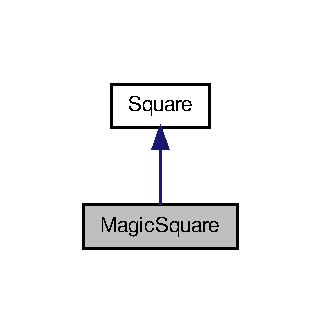
\includegraphics[width=154pt]{classMagicSquare__inherit__graph}
\end{center}
\end{figure}


Collaboration diagram for Magic\-Square\-:\nopagebreak
\begin{figure}[H]
\begin{center}
\leavevmode
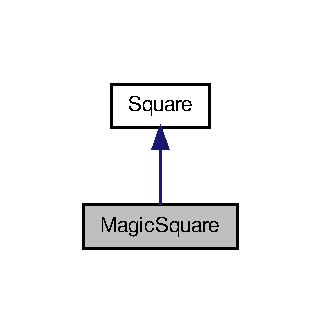
\includegraphics[width=154pt]{classMagicSquare__coll__graph}
\end{center}
\end{figure}
\subsection*{Public Member Functions}
\begin{DoxyCompactItemize}
\item 
\hyperlink{classMagicSquare_ad0c3bd76077df9027cbc7001320546f4}{Magic\-Square} ()
\item 
\hyperlink{classMagicSquare_a44538ecf1867db5ee72f4efa03bae693}{Magic\-Square} (int a\-\_\-ordinal)  throw (const invalid\-\_\-argument)
\item 
\hyperlink{classMagicSquare}{Magic\-Square} \hyperlink{classMagicSquare_a1e8210cf322013adacfb074b0a05cdb7}{switch\-\_\-rows} (int index)  throw (const out\-\_\-of\-\_\-range)
\item 
\hyperlink{classMagicSquare}{Magic\-Square} \hyperlink{classMagicSquare_a6850cf9ba88d20b8a28b9972f020a67a}{switch\-\_\-columns} (int index)  throw (const out\-\_\-of\-\_\-range)
\item 
\hyperlink{classMagicSquare}{Magic\-Square} \hyperlink{classMagicSquare_a3a2c8af100b50506625a8a834a37beb8}{switch\-\_\-diagonal\-\_\-top\-\_\-left} ()
\item 
\hyperlink{classMagicSquare}{Magic\-Square} \hyperlink{classMagicSquare_addc82eb3e9deef9d557a1cb2680b5c1b}{switch\-\_\-diagonal\-\_\-top\-\_\-right} ()
\item 
\hyperlink{classMagicSquare}{Magic\-Square} \hyperlink{classMagicSquare_adbab741c88ad073b2125c5499f7fdca3}{rotate\-\_\-90} ()
\item 
int \hyperlink{classMagicSquare_aff24d6b2c5b224f428db87bf35fa81b7}{get\-\_\-magic\-\_\-number} () const 
\item 
string \hyperlink{classMagicSquare_aa88327706850d00fa8de80b85e7c68c9}{str} () const 
\end{DoxyCompactItemize}
\subsection*{Additional Inherited Members}


\subsection{Detailed Description}
Difinition of a \hyperlink{classMagicSquare}{Magic\-Square}. Has all the algorithms to generate a \hyperlink{classMagicSquare}{Magic\-Square} out of a ordinal number and also to mutate the basic \hyperlink{classMagicSquare}{Magic\-Square} to other valid Magic\-Squares. 

\subsection{Constructor \& Destructor Documentation}
\hypertarget{classMagicSquare_ad0c3bd76077df9027cbc7001320546f4}{\index{Magic\-Square@{Magic\-Square}!Magic\-Square@{Magic\-Square}}
\index{Magic\-Square@{Magic\-Square}!MagicSquare@{Magic\-Square}}
\subsubsection[{Magic\-Square}]{\setlength{\rightskip}{0pt plus 5cm}Magic\-Square\-::\-Magic\-Square (
\begin{DoxyParamCaption}
{}
\end{DoxyParamCaption}
)}}\label{classMagicSquare_ad0c3bd76077df9027cbc7001320546f4}
Default constructor. Initializises a \hyperlink{classMagicSquare}{Magic\-Square} with an ordinal number of 5. \hypertarget{classMagicSquare_a44538ecf1867db5ee72f4efa03bae693}{\index{Magic\-Square@{Magic\-Square}!Magic\-Square@{Magic\-Square}}
\index{Magic\-Square@{Magic\-Square}!MagicSquare@{Magic\-Square}}
\subsubsection[{Magic\-Square}]{\setlength{\rightskip}{0pt plus 5cm}Magic\-Square\-::\-Magic\-Square (
\begin{DoxyParamCaption}
\item[{int}]{a\-\_\-ordinal}
\end{DoxyParamCaption}
)  throw (const invalid\-\_\-argument)}}\label{classMagicSquare_a44538ecf1867db5ee72f4efa03bae693}
Initializies a \hyperlink{classMagicSquare}{Magic\-Square} with a odd ordnial number.


\begin{DoxyParams}{Parameters}
{\em a\-\_\-ordinal} & The ordinal number of the \hyperlink{classMagicSquare}{Magic\-Square}.\\
\hline
\end{DoxyParams}

\begin{DoxyExceptions}{Exceptions}
{\em const} & invalid\-\_\-argument when ordinal number is even. \\
\hline
\end{DoxyExceptions}


\subsection{Member Function Documentation}
\hypertarget{classMagicSquare_aff24d6b2c5b224f428db87bf35fa81b7}{\index{Magic\-Square@{Magic\-Square}!get\-\_\-magic\-\_\-number@{get\-\_\-magic\-\_\-number}}
\index{get\-\_\-magic\-\_\-number@{get\-\_\-magic\-\_\-number}!MagicSquare@{Magic\-Square}}
\subsubsection[{get\-\_\-magic\-\_\-number}]{\setlength{\rightskip}{0pt plus 5cm}int Magic\-Square\-::get\-\_\-magic\-\_\-number (
\begin{DoxyParamCaption}
{}
\end{DoxyParamCaption}
) const}}\label{classMagicSquare_aff24d6b2c5b224f428db87bf35fa81b7}
Calculates and returns the magic number of the \hyperlink{classMagicSquare}{Magic\-Square}.

\begin{DoxyReturn}{Returns}
the magic number of the \hyperlink{classMagicSquare}{Magic\-Square}. 
\end{DoxyReturn}
\hypertarget{classMagicSquare_adbab741c88ad073b2125c5499f7fdca3}{\index{Magic\-Square@{Magic\-Square}!rotate\-\_\-90@{rotate\-\_\-90}}
\index{rotate\-\_\-90@{rotate\-\_\-90}!MagicSquare@{Magic\-Square}}
\subsubsection[{rotate\-\_\-90}]{\setlength{\rightskip}{0pt plus 5cm}{\bf Magic\-Square} Magic\-Square\-::rotate\-\_\-90 (
\begin{DoxyParamCaption}
{}
\end{DoxyParamCaption}
)}}\label{classMagicSquare_adbab741c88ad073b2125c5499f7fdca3}
Rotates a \hyperlink{classMagicSquare}{Magic\-Square} 90 degrees in clockwise direction.

\begin{DoxyReturn}{Returns}
a new \hyperlink{classMagicSquare}{Magic\-Square} rotated 90 degrees clockwise. 
\end{DoxyReturn}
\hypertarget{classMagicSquare_aa88327706850d00fa8de80b85e7c68c9}{\index{Magic\-Square@{Magic\-Square}!str@{str}}
\index{str@{str}!MagicSquare@{Magic\-Square}}
\subsubsection[{str}]{\setlength{\rightskip}{0pt plus 5cm}string Magic\-Square\-::str (
\begin{DoxyParamCaption}
{}
\end{DoxyParamCaption}
) const}}\label{classMagicSquare_aa88327706850d00fa8de80b85e7c68c9}
Generates and returns the string representation of a \hyperlink{classMagicSquare}{Magic\-Square}. \par
\par
 11 2 25 18 9\par
 23 14 7 5 16\par
 4 20 13 6 22\par
 10 21 19 12 3\par
 17 8 1 24 15\par


\begin{DoxyReturn}{Returns}
string representation fo a Magic\-Scrqare. 
\end{DoxyReturn}
\hypertarget{classMagicSquare_a6850cf9ba88d20b8a28b9972f020a67a}{\index{Magic\-Square@{Magic\-Square}!switch\-\_\-columns@{switch\-\_\-columns}}
\index{switch\-\_\-columns@{switch\-\_\-columns}!MagicSquare@{Magic\-Square}}
\subsubsection[{switch\-\_\-columns}]{\setlength{\rightskip}{0pt plus 5cm}{\bf Magic\-Square} Magic\-Square\-::switch\-\_\-columns (
\begin{DoxyParamCaption}
\item[{int}]{index}
\end{DoxyParamCaption}
)  throw (const out\-\_\-of\-\_\-range)}}\label{classMagicSquare_a6850cf9ba88d20b8a28b9972f020a67a}
Switches two columns which have the same distance from the center.


\begin{DoxyParams}{Parameters}
{\em index} & Distance form left/right border.\\
\hline
\end{DoxyParams}
\begin{DoxyReturn}{Returns}
a new \hyperlink{classMagicSquare}{Magic\-Square} with switched columns.
\end{DoxyReturn}

\begin{DoxyExceptions}{Exceptions}
{\em const} & out\-\_\-of\-\_\-range when index is not valid. \\
\hline
\end{DoxyExceptions}
\hypertarget{classMagicSquare_a3a2c8af100b50506625a8a834a37beb8}{\index{Magic\-Square@{Magic\-Square}!switch\-\_\-diagonal\-\_\-top\-\_\-left@{switch\-\_\-diagonal\-\_\-top\-\_\-left}}
\index{switch\-\_\-diagonal\-\_\-top\-\_\-left@{switch\-\_\-diagonal\-\_\-top\-\_\-left}!MagicSquare@{Magic\-Square}}
\subsubsection[{switch\-\_\-diagonal\-\_\-top\-\_\-left}]{\setlength{\rightskip}{0pt plus 5cm}{\bf Magic\-Square} Magic\-Square\-::switch\-\_\-diagonal\-\_\-top\-\_\-left (
\begin{DoxyParamCaption}
{}
\end{DoxyParamCaption}
)}}\label{classMagicSquare_a3a2c8af100b50506625a8a834a37beb8}
Mirrors the \hyperlink{classMagicSquare}{Magic\-Square} at the diagonal line form top left to bottom right.

\begin{DoxyReturn}{Returns}
a new \hyperlink{classMagicSquare}{Magic\-Square} mirrored at the diagonal. 
\end{DoxyReturn}
\hypertarget{classMagicSquare_addc82eb3e9deef9d557a1cb2680b5c1b}{\index{Magic\-Square@{Magic\-Square}!switch\-\_\-diagonal\-\_\-top\-\_\-right@{switch\-\_\-diagonal\-\_\-top\-\_\-right}}
\index{switch\-\_\-diagonal\-\_\-top\-\_\-right@{switch\-\_\-diagonal\-\_\-top\-\_\-right}!MagicSquare@{Magic\-Square}}
\subsubsection[{switch\-\_\-diagonal\-\_\-top\-\_\-right}]{\setlength{\rightskip}{0pt plus 5cm}{\bf Magic\-Square} Magic\-Square\-::switch\-\_\-diagonal\-\_\-top\-\_\-right (
\begin{DoxyParamCaption}
{}
\end{DoxyParamCaption}
)}}\label{classMagicSquare_addc82eb3e9deef9d557a1cb2680b5c1b}
Mirrors the \hyperlink{classMagicSquare}{Magic\-Square} at the diagonal line form top right to bottom left.

\begin{DoxyReturn}{Returns}
a new \hyperlink{classMagicSquare}{Magic\-Square} mirrored at the diagonal. 
\end{DoxyReturn}
\hypertarget{classMagicSquare_a1e8210cf322013adacfb074b0a05cdb7}{\index{Magic\-Square@{Magic\-Square}!switch\-\_\-rows@{switch\-\_\-rows}}
\index{switch\-\_\-rows@{switch\-\_\-rows}!MagicSquare@{Magic\-Square}}
\subsubsection[{switch\-\_\-rows}]{\setlength{\rightskip}{0pt plus 5cm}{\bf Magic\-Square} Magic\-Square\-::switch\-\_\-rows (
\begin{DoxyParamCaption}
\item[{int}]{index}
\end{DoxyParamCaption}
)  throw (const out\-\_\-of\-\_\-range)}}\label{classMagicSquare_a1e8210cf322013adacfb074b0a05cdb7}
Switches two rows which have the same distance from the center.


\begin{DoxyParams}{Parameters}
{\em index} & Distance form top/bottom border.\\
\hline
\end{DoxyParams}
\begin{DoxyReturn}{Returns}
a new \hyperlink{classMagicSquare}{Magic\-Square} with switched rows.
\end{DoxyReturn}

\begin{DoxyExceptions}{Exceptions}
{\em const} & out\-\_\-of\-\_\-range when index is not valid. \\
\hline
\end{DoxyExceptions}


The documentation for this class was generated from the following files\-:\begin{DoxyCompactItemize}
\item 
\hyperlink{magic__square_8h}{magic\-\_\-square.\-h}\item 
\hyperlink{magic__square_8cpp}{magic\-\_\-square.\-cpp}\end{DoxyCompactItemize}

\hypertarget{classMagicSquareSet}{\section{Magic\-Square\-Set Class Reference}
\label{classMagicSquareSet}\index{Magic\-Square\-Set@{Magic\-Square\-Set}}
}


{\ttfamily \#include $<$magic\-\_\-square\-\_\-set.\-h$>$}

\subsection*{Public Member Functions}
\begin{DoxyCompactItemize}
\item 
\hyperlink{classMagicSquareSet_a70591cbccd41666cce19f2d720904162}{Magic\-Square\-Set} ()
\item 
\hyperlink{classMagicSquareSet_a6b537e36c455af04096353045a3b2d92}{Magic\-Square\-Set} (const \hyperlink{classMagicSquareSet}{Magic\-Square\-Set} \&original)
\item 
virtual \hyperlink{classMagicSquareSet_adfe49757d5627696c83c3fbf903b7665}{$\sim$\-Magic\-Square\-Set} ()
\item 
int \hyperlink{classMagicSquareSet_af6d417c4a64ad109b86a20cc7499e378}{add} (\hyperlink{classMagicSquare}{Magic\-Square} $\ast$a\-\_\-magic\-\_\-square)
\item 
int \hyperlink{classMagicSquareSet_a7e44d044af79459d650e19fa564c00b5}{size} () const 
\item 
string \hyperlink{classMagicSquareSet_a313f7b06fb202ab327639fedaeda8b03}{str} () const 
\item 
\hyperlink{classMagicSquareSet}{Magic\-Square\-Set} \& \hyperlink{classMagicSquareSet_a219ab922ac0c556c11134a2cbeb2f761}{operator=} (const \hyperlink{classMagicSquareSet}{Magic\-Square\-Set} \&other)
\item 
\hyperlink{classMagicSquare}{Magic\-Square} \hyperlink{classMagicSquareSet_a2ae62f09ce34696ee5bbdb9930b92c85}{operator\mbox{[}$\,$\mbox{]}} (int key) const 
\end{DoxyCompactItemize}


\subsection{Constructor \& Destructor Documentation}
\hypertarget{classMagicSquareSet_a70591cbccd41666cce19f2d720904162}{\index{Magic\-Square\-Set@{Magic\-Square\-Set}!Magic\-Square\-Set@{Magic\-Square\-Set}}
\index{Magic\-Square\-Set@{Magic\-Square\-Set}!MagicSquareSet@{Magic\-Square\-Set}}
\subsubsection[{Magic\-Square\-Set}]{\setlength{\rightskip}{0pt plus 5cm}Magic\-Square\-Set\-::\-Magic\-Square\-Set (
\begin{DoxyParamCaption}
{}
\end{DoxyParamCaption}
)}}\label{classMagicSquareSet_a70591cbccd41666cce19f2d720904162}
Default constructor. Initializes a empty vectors of squares. \hypertarget{classMagicSquareSet_a6b537e36c455af04096353045a3b2d92}{\index{Magic\-Square\-Set@{Magic\-Square\-Set}!Magic\-Square\-Set@{Magic\-Square\-Set}}
\index{Magic\-Square\-Set@{Magic\-Square\-Set}!MagicSquareSet@{Magic\-Square\-Set}}
\subsubsection[{Magic\-Square\-Set}]{\setlength{\rightskip}{0pt plus 5cm}Magic\-Square\-Set\-::\-Magic\-Square\-Set (
\begin{DoxyParamCaption}
\item[{const {\bf Magic\-Square\-Set} \&}]{original}
\end{DoxyParamCaption}
)}}\label{classMagicSquareSet_a6b537e36c455af04096353045a3b2d92}
Copy-\/constructor for a \hyperlink{classMagicSquareSet}{Magic\-Square\-Set}. Implements the deep copy.


\begin{DoxyParams}{Parameters}
{\em original} & The \hyperlink{classMagicSquareSet}{Magic\-Square\-Set} to copy from. \\
\hline
\end{DoxyParams}
\hypertarget{classMagicSquareSet_adfe49757d5627696c83c3fbf903b7665}{\index{Magic\-Square\-Set@{Magic\-Square\-Set}!$\sim$\-Magic\-Square\-Set@{$\sim$\-Magic\-Square\-Set}}
\index{$\sim$\-Magic\-Square\-Set@{$\sim$\-Magic\-Square\-Set}!MagicSquareSet@{Magic\-Square\-Set}}
\subsubsection[{$\sim$\-Magic\-Square\-Set}]{\setlength{\rightskip}{0pt plus 5cm}Magic\-Square\-Set\-::$\sim$\-Magic\-Square\-Set (
\begin{DoxyParamCaption}
{}
\end{DoxyParamCaption}
)\hspace{0.3cm}{\ttfamily [virtual]}}}\label{classMagicSquareSet_adfe49757d5627696c83c3fbf903b7665}
Deconstructor for the \hyperlink{classMagicSquareSet}{Magic\-Square\-Set}. 

\subsection{Member Function Documentation}
\hypertarget{classMagicSquareSet_af6d417c4a64ad109b86a20cc7499e378}{\index{Magic\-Square\-Set@{Magic\-Square\-Set}!add@{add}}
\index{add@{add}!MagicSquareSet@{Magic\-Square\-Set}}
\subsubsection[{add}]{\setlength{\rightskip}{0pt plus 5cm}int Magic\-Square\-Set\-::add (
\begin{DoxyParamCaption}
\item[{{\bf Magic\-Square} $\ast$}]{a\-\_\-magic\-\_\-square}
\end{DoxyParamCaption}
)}}\label{classMagicSquareSet_af6d417c4a64ad109b86a20cc7499e378}
Adds a \hyperlink{classMagicSquare}{Magic\-Square} to the set when it's not already in the set. When its already in the set, it just ignores it.


\begin{DoxyParams}{Parameters}
{\em a\-\_\-magic\-\_\-square} & The \hyperlink{classMagicSquare}{Magic\-Square} to add to the set.\\
\hline
\end{DoxyParams}
\begin{DoxyReturn}{Returns}
the new size of the set. 
\end{DoxyReturn}
\hypertarget{classMagicSquareSet_a219ab922ac0c556c11134a2cbeb2f761}{\index{Magic\-Square\-Set@{Magic\-Square\-Set}!operator=@{operator=}}
\index{operator=@{operator=}!MagicSquareSet@{Magic\-Square\-Set}}
\subsubsection[{operator=}]{\setlength{\rightskip}{0pt plus 5cm}{\bf Magic\-Square\-Set} \& Magic\-Square\-Set\-::operator= (
\begin{DoxyParamCaption}
\item[{const {\bf Magic\-Square\-Set} \&}]{other}
\end{DoxyParamCaption}
)}}\label{classMagicSquareSet_a219ab922ac0c556c11134a2cbeb2f761}
Overloads the assignment operator=. Defines how to assign a \hyperlink{classMagicSquareSet}{Magic\-Square\-Set} to an other.


\begin{DoxyParams}{Parameters}
{\em other} & The \hyperlink{classMagicSquareSet}{Magic\-Square\-Set} to assign.\\
\hline
\end{DoxyParams}
\begin{DoxyReturn}{Returns}
The actual \hyperlink{classMagicSquareSet}{Magic\-Square\-Set}. 
\end{DoxyReturn}


Here is the call graph for this function\-:\nopagebreak
\begin{figure}[H]
\begin{center}
\leavevmode
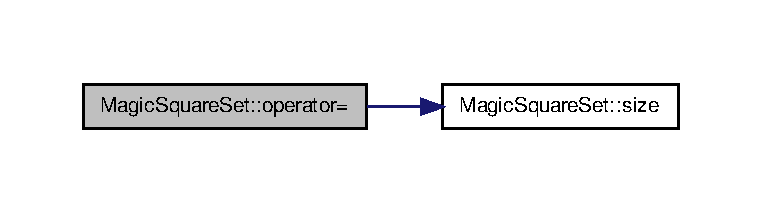
\includegraphics[width=350pt]{classMagicSquareSet_a219ab922ac0c556c11134a2cbeb2f761_cgraph}
\end{center}
\end{figure}


\hypertarget{classMagicSquareSet_a2ae62f09ce34696ee5bbdb9930b92c85}{\index{Magic\-Square\-Set@{Magic\-Square\-Set}!operator\mbox{[}$\,$\mbox{]}@{operator[]}}
\index{operator\mbox{[}$\,$\mbox{]}@{operator[]}!MagicSquareSet@{Magic\-Square\-Set}}
\subsubsection[{operator[]}]{\setlength{\rightskip}{0pt plus 5cm}{\bf Magic\-Square} Magic\-Square\-Set\-::operator\mbox{[}$\,$\mbox{]} (
\begin{DoxyParamCaption}
\item[{int}]{key}
\end{DoxyParamCaption}
) const}}\label{classMagicSquareSet_a2ae62f09ce34696ee5bbdb9930b92c85}
Returns a \hyperlink{classMagicSquare}{Magic\-Square}, saved at the position of a key.


\begin{DoxyParams}{Parameters}
{\em key} & Key of the \hyperlink{classMagicSquare}{Magic\-Square} to access.\\
\hline
\end{DoxyParams}
\begin{DoxyReturn}{Returns}
the \hyperlink{classMagicSquare}{Magic\-Square} at the position of key. 
\end{DoxyReturn}
\hypertarget{classMagicSquareSet_a7e44d044af79459d650e19fa564c00b5}{\index{Magic\-Square\-Set@{Magic\-Square\-Set}!size@{size}}
\index{size@{size}!MagicSquareSet@{Magic\-Square\-Set}}
\subsubsection[{size}]{\setlength{\rightskip}{0pt plus 5cm}int Magic\-Square\-Set\-::size (
\begin{DoxyParamCaption}
{}
\end{DoxyParamCaption}
) const}}\label{classMagicSquareSet_a7e44d044af79459d650e19fa564c00b5}
Returns the size of the set.

\begin{DoxyReturn}{Returns}
size of the set. 
\end{DoxyReturn}
\hypertarget{classMagicSquareSet_a313f7b06fb202ab327639fedaeda8b03}{\index{Magic\-Square\-Set@{Magic\-Square\-Set}!str@{str}}
\index{str@{str}!MagicSquareSet@{Magic\-Square\-Set}}
\subsubsection[{str}]{\setlength{\rightskip}{0pt plus 5cm}string Magic\-Square\-Set\-::str (
\begin{DoxyParamCaption}
{}
\end{DoxyParamCaption}
) const}}\label{classMagicSquareSet_a313f7b06fb202ab327639fedaeda8b03}
Generates and returns the string representation of a set. \par
\par
 11 2 25 18 9\par
 23 14 7 5 16\par
 4 20 13 6 22\par
 10 21 19 12 3\par
 17 8 1 24 15\par
 \par
 11 2 25 18 9\par
 23 14 7 5 16\par
 4 20 13 6 22\par
 10 21 19 12 3\par
 17 8 1 24 15\par
 \par
 Ordnung\-: 5 Anzahl\-: 2 Magic number\-: 65

\begin{DoxyReturn}{Returns}
the string representation of a set. 
\end{DoxyReturn}


Here is the call graph for this function\-:\nopagebreak
\begin{figure}[H]
\begin{center}
\leavevmode
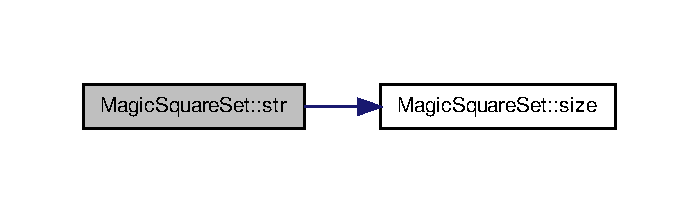
\includegraphics[width=336pt]{classMagicSquareSet_a313f7b06fb202ab327639fedaeda8b03_cgraph}
\end{center}
\end{figure}




The documentation for this class was generated from the following files\-:\begin{DoxyCompactItemize}
\item 
\hyperlink{magic__square__set_8h}{magic\-\_\-square\-\_\-set.\-h}\item 
\hyperlink{magic__square__set_8cpp}{magic\-\_\-square\-\_\-set.\-cpp}\end{DoxyCompactItemize}

\hypertarget{classSquare}{\section{Square Class Reference}
\label{classSquare}\index{Square@{Square}}
}


{\ttfamily \#include $<$square.\-h$>$}



Inheritance diagram for Square\-:\nopagebreak
\begin{figure}[H]
\begin{center}
\leavevmode
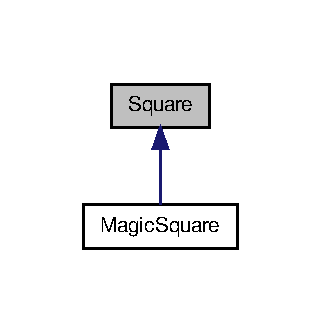
\includegraphics[width=154pt]{classSquare__inherit__graph}
\end{center}
\end{figure}
\subsection*{Public Member Functions}
\begin{DoxyCompactItemize}
\item 
\hyperlink{classSquare_a3dc7ff9aefc2725172b5d3153973d243}{Square} ()
\item 
\hyperlink{classSquare_a687fd93a7b5b6f4e310dda4765f2e4b9}{Square} (int the\-\_\-ordinal)
\item 
\hyperlink{classSquare_a5b24c398bbcd2fa54d750e821b682be4}{Square} (const \hyperlink{classSquare}{Square} \&original)
\item 
\hyperlink{classSquare_ab2ce549e03ee04a325fde6fa69b0bd56}{Square} (int the\-\_\-ordinal, int $\ast$$\ast$the\-\_\-data)
\item 
\hyperlink{classSquare_a6aaedd8907eb79371c1a964c22a91df1}{Square} (int the\-\_\-ordinal, string the\-\_\-data)  throw (const invalid\-\_\-argument)
\item 
virtual \hyperlink{classSquare_a90af7ce1060cff7b717ceddb333846b8}{$\sim$\-Square} ()
\item 
int \hyperlink{classSquare_aa88af87efb77891af13d7e51875c8a4d}{get\-\_\-ordinal} () const 
\item 
\hyperlink{classSquare}{Square} \& \hyperlink{classSquare_aefd7f1993a8a7dc2da19773aa615d4e5}{operator=} (const \hyperlink{classSquare}{Square} \&other)
\item 
int $\ast$ \hyperlink{classSquare_a7dfc1c4829599e231ad72d1f2b6d0e83}{operator\mbox{[}$\,$\mbox{]}} (const int \&key) const 
\item 
bool \hyperlink{classSquare_a68344a4bfb9a5bc8b6382f302049ec6f}{operator==} (const \hyperlink{classSquare}{Square} \&other) const 
\item 
bool \hyperlink{classSquare_a62325c38089124501ce08ddf2fb7a4eb}{operator!=} (const \hyperlink{classSquare}{Square} \&other) const 
\end{DoxyCompactItemize}
\subsection*{Protected Member Functions}
\begin{DoxyCompactItemize}
\item 
void \hyperlink{classSquare_af7e972a99bbd1229c1a2ed9c9973b1a3}{init} ()
\item 
void \hyperlink{classSquare_ad8a97711bb0377c85707f926c715149a}{init} (int $\ast$$\ast$the\-\_\-data)
\item 
void \hyperlink{classSquare_a613cdeed3d18a22bd212431d0c1d3b3d}{clear} ()
\end{DoxyCompactItemize}
\subsection*{Protected Attributes}
\begin{DoxyCompactItemize}
\item 
int \hyperlink{classSquare_abfaf02c2958d841dc7def09197d26d93}{ordinal}
\item 
int $\ast$$\ast$ \hyperlink{classSquare_a3b5a8a3e9ae6e0570dd54ab360bacef0}{data}
\end{DoxyCompactItemize}


\subsection{Detailed Description}
Definition of the Class \hyperlink{classSquare}{Square}. A \hyperlink{classSquare}{Square} is a array where the columns and the rows have the same size. 

\subsection{Constructor \& Destructor Documentation}
\hypertarget{classSquare_a3dc7ff9aefc2725172b5d3153973d243}{\index{Square@{Square}!Square@{Square}}
\index{Square@{Square}!Square@{Square}}
\subsubsection[{Square}]{\setlength{\rightskip}{0pt plus 5cm}Square\-::\-Square (
\begin{DoxyParamCaption}
{}
\end{DoxyParamCaption}
)}}\label{classSquare_a3dc7ff9aefc2725172b5d3153973d243}
Initializes a \hyperlink{classSquare}{Square} with the ordinal number 9. 

Here is the call graph for this function\-:\nopagebreak
\begin{figure}[H]
\begin{center}
\leavevmode
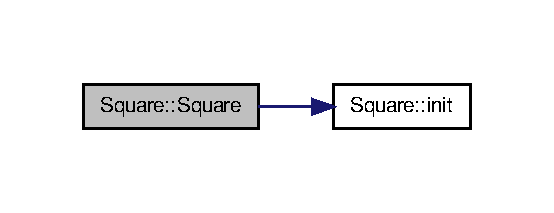
\includegraphics[width=266pt]{classSquare_a3dc7ff9aefc2725172b5d3153973d243_cgraph}
\end{center}
\end{figure}


\hypertarget{classSquare_a687fd93a7b5b6f4e310dda4765f2e4b9}{\index{Square@{Square}!Square@{Square}}
\index{Square@{Square}!Square@{Square}}
\subsubsection[{Square}]{\setlength{\rightskip}{0pt plus 5cm}Square\-::\-Square (
\begin{DoxyParamCaption}
\item[{int}]{the\-\_\-ordinal}
\end{DoxyParamCaption}
)}}\label{classSquare_a687fd93a7b5b6f4e310dda4765f2e4b9}
Initializes a \hyperlink{classSquare}{Square} with a given ordinal number.


\begin{DoxyParams}{Parameters}
{\em the\-\_\-ordinal} & Ordinal number of the square. \\
\hline
\end{DoxyParams}


Here is the call graph for this function\-:\nopagebreak
\begin{figure}[H]
\begin{center}
\leavevmode
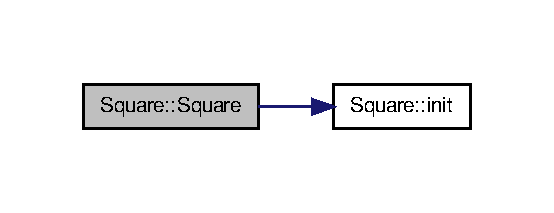
\includegraphics[width=266pt]{classSquare_a687fd93a7b5b6f4e310dda4765f2e4b9_cgraph}
\end{center}
\end{figure}


\hypertarget{classSquare_a5b24c398bbcd2fa54d750e821b682be4}{\index{Square@{Square}!Square@{Square}}
\index{Square@{Square}!Square@{Square}}
\subsubsection[{Square}]{\setlength{\rightskip}{0pt plus 5cm}Square\-::\-Square (
\begin{DoxyParamCaption}
\item[{const {\bf Square} \&}]{original}
\end{DoxyParamCaption}
)}}\label{classSquare_a5b24c398bbcd2fa54d750e821b682be4}
copy-\/constructor.


\begin{DoxyParams}{Parameters}
{\em original} & The \hyperlink{classSquare}{Square} to copy. \\
\hline
\end{DoxyParams}


Here is the call graph for this function\-:\nopagebreak
\begin{figure}[H]
\begin{center}
\leavevmode
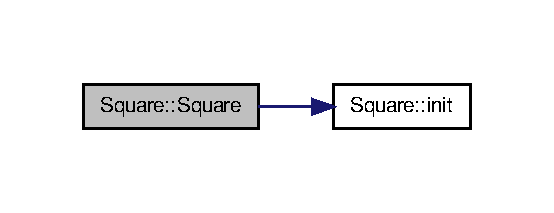
\includegraphics[width=266pt]{classSquare_a5b24c398bbcd2fa54d750e821b682be4_cgraph}
\end{center}
\end{figure}


\hypertarget{classSquare_ab2ce549e03ee04a325fde6fa69b0bd56}{\index{Square@{Square}!Square@{Square}}
\index{Square@{Square}!Square@{Square}}
\subsubsection[{Square}]{\setlength{\rightskip}{0pt plus 5cm}Square\-::\-Square (
\begin{DoxyParamCaption}
\item[{int}]{the\-\_\-ordinal, }
\item[{int $\ast$$\ast$}]{the\-\_\-data}
\end{DoxyParamCaption}
)}}\label{classSquare_ab2ce549e03ee04a325fde6fa69b0bd56}
Initializes a \hyperlink{classSquare}{Square} with a given ordinal number and a given dataset.


\begin{DoxyParams}{Parameters}
{\em the\-\_\-ordinal} & Ordinal number of the \hyperlink{classSquare}{Square}. \\
\hline
{\em the\-\_\-data} & Data for the \hyperlink{classSquare}{Square}. \\
\hline
\end{DoxyParams}


Here is the call graph for this function\-:\nopagebreak
\begin{figure}[H]
\begin{center}
\leavevmode
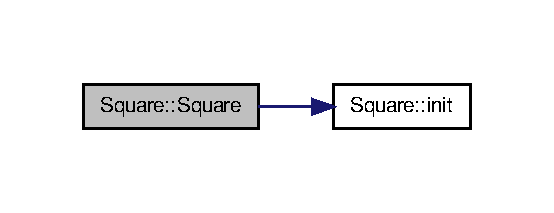
\includegraphics[width=266pt]{classSquare_ab2ce549e03ee04a325fde6fa69b0bd56_cgraph}
\end{center}
\end{figure}


\hypertarget{classSquare_a6aaedd8907eb79371c1a964c22a91df1}{\index{Square@{Square}!Square@{Square}}
\index{Square@{Square}!Square@{Square}}
\subsubsection[{Square}]{\setlength{\rightskip}{0pt plus 5cm}Square\-::\-Square (
\begin{DoxyParamCaption}
\item[{int}]{the\-\_\-ordinal, }
\item[{string}]{the\-\_\-data}
\end{DoxyParamCaption}
)  throw (const invalid\-\_\-argument)}}\label{classSquare_a6aaedd8907eb79371c1a964c22a91df1}
Initializes a \hyperlink{classSquare}{Square} with a given ordinal number and a given dataset as string out of numbers.


\begin{DoxyParams}{Parameters}
{\em the\-\_\-ordinal} & Ordinal number of the \hyperlink{classSquare}{Square}. \\
\hline
{\em the\-\_\-data} & Data for the \hyperlink{classSquare}{Square}.\\
\hline
\end{DoxyParams}

\begin{DoxyExceptions}{Exceptions}
{\em const} & invalid\-\_\-argument when the ordinal and data are not consistent. \\
\hline
\end{DoxyExceptions}
\hypertarget{classSquare_a90af7ce1060cff7b717ceddb333846b8}{\index{Square@{Square}!$\sim$\-Square@{$\sim$\-Square}}
\index{$\sim$\-Square@{$\sim$\-Square}!Square@{Square}}
\subsubsection[{$\sim$\-Square}]{\setlength{\rightskip}{0pt plus 5cm}Square\-::$\sim$\-Square (
\begin{DoxyParamCaption}
{}
\end{DoxyParamCaption}
)\hspace{0.3cm}{\ttfamily [virtual]}}}\label{classSquare_a90af7ce1060cff7b717ceddb333846b8}
Deconstructor. Clears the heap. 

Here is the call graph for this function\-:\nopagebreak
\begin{figure}[H]
\begin{center}
\leavevmode
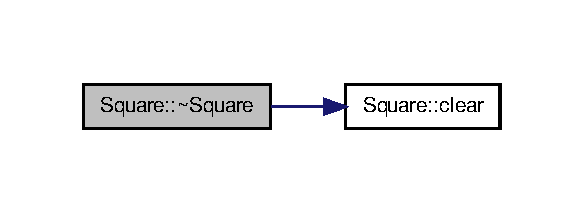
\includegraphics[width=280pt]{classSquare_a90af7ce1060cff7b717ceddb333846b8_cgraph}
\end{center}
\end{figure}




\subsection{Member Function Documentation}
\hypertarget{classSquare_a613cdeed3d18a22bd212431d0c1d3b3d}{\index{Square@{Square}!clear@{clear}}
\index{clear@{clear}!Square@{Square}}
\subsubsection[{clear}]{\setlength{\rightskip}{0pt plus 5cm}void Square\-::clear (
\begin{DoxyParamCaption}
{}
\end{DoxyParamCaption}
)\hspace{0.3cm}{\ttfamily [protected]}}}\label{classSquare_a613cdeed3d18a22bd212431d0c1d3b3d}
Cleans the square and its sub arrays form memory. \hypertarget{classSquare_aa88af87efb77891af13d7e51875c8a4d}{\index{Square@{Square}!get\-\_\-ordinal@{get\-\_\-ordinal}}
\index{get\-\_\-ordinal@{get\-\_\-ordinal}!Square@{Square}}
\subsubsection[{get\-\_\-ordinal}]{\setlength{\rightskip}{0pt plus 5cm}int Square\-::get\-\_\-ordinal (
\begin{DoxyParamCaption}
{}
\end{DoxyParamCaption}
) const}}\label{classSquare_aa88af87efb77891af13d7e51875c8a4d}
Returns the ordinal of the \hyperlink{classSquare}{Square}.

\begin{DoxyReturn}{Returns}
ordinal of the square. 
\end{DoxyReturn}
\hypertarget{classSquare_af7e972a99bbd1229c1a2ed9c9973b1a3}{\index{Square@{Square}!init@{init}}
\index{init@{init}!Square@{Square}}
\subsubsection[{init}]{\setlength{\rightskip}{0pt plus 5cm}void Square\-::init (
\begin{DoxyParamCaption}
{}
\end{DoxyParamCaption}
)\hspace{0.3cm}{\ttfamily [protected]}}}\label{classSquare_af7e972a99bbd1229c1a2ed9c9973b1a3}
Initializes an empty square. (filled with 0) \hypertarget{classSquare_ad8a97711bb0377c85707f926c715149a}{\index{Square@{Square}!init@{init}}
\index{init@{init}!Square@{Square}}
\subsubsection[{init}]{\setlength{\rightskip}{0pt plus 5cm}void Square\-::init (
\begin{DoxyParamCaption}
\item[{int $\ast$$\ast$}]{the\-\_\-data}
\end{DoxyParamCaption}
)\hspace{0.3cm}{\ttfamily [protected]}}}\label{classSquare_ad8a97711bb0377c85707f926c715149a}
Initializes the square with a given 2d array.


\begin{DoxyParams}{Parameters}
{\em the\-\_\-data} & the data to fill the \hyperlink{classSquare}{Square}. \\
\hline
\end{DoxyParams}
\hypertarget{classSquare_a62325c38089124501ce08ddf2fb7a4eb}{\index{Square@{Square}!operator!=@{operator!=}}
\index{operator!=@{operator!=}!Square@{Square}}
\subsubsection[{operator!=}]{\setlength{\rightskip}{0pt plus 5cm}bool Square\-::operator!= (
\begin{DoxyParamCaption}
\item[{const {\bf Square} \&}]{other}
\end{DoxyParamCaption}
) const}}\label{classSquare_a62325c38089124501ce08ddf2fb7a4eb}
Overloads the operator!=. Checks if a \hyperlink{classMagicSquare}{Magic\-Square} is not equal an other.


\begin{DoxyParams}{Parameters}
{\em other} & Other \hyperlink{classMagicSquare}{Magic\-Square} to compare.\\
\hline
\end{DoxyParams}
\begin{DoxyReturn}{Returns}
true when they are not equal. false when they are equal. 
\end{DoxyReturn}
\hypertarget{classSquare_aefd7f1993a8a7dc2da19773aa615d4e5}{\index{Square@{Square}!operator=@{operator=}}
\index{operator=@{operator=}!Square@{Square}}
\subsubsection[{operator=}]{\setlength{\rightskip}{0pt plus 5cm}{\bf Square} \& Square\-::operator= (
\begin{DoxyParamCaption}
\item[{const {\bf Square} \&}]{other}
\end{DoxyParamCaption}
)}}\label{classSquare_aefd7f1993a8a7dc2da19773aa615d4e5}
Overloads assignment operator=. Defines how to copy a \hyperlink{classSquare}{Square} to an other.


\begin{DoxyParams}{Parameters}
{\em other} & The square to copy.\\
\hline
\end{DoxyParams}
\begin{DoxyReturn}{Returns}
a reference to itself. 
\end{DoxyReturn}


Here is the call graph for this function\-:\nopagebreak
\begin{figure}[H]
\begin{center}
\leavevmode
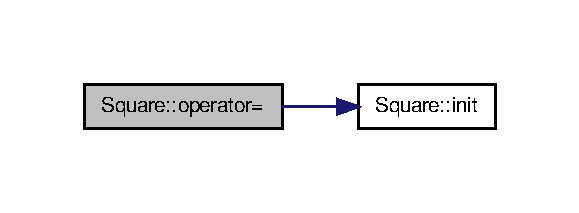
\includegraphics[width=278pt]{classSquare_aefd7f1993a8a7dc2da19773aa615d4e5_cgraph}
\end{center}
\end{figure}


\hypertarget{classSquare_a68344a4bfb9a5bc8b6382f302049ec6f}{\index{Square@{Square}!operator==@{operator==}}
\index{operator==@{operator==}!Square@{Square}}
\subsubsection[{operator==}]{\setlength{\rightskip}{0pt plus 5cm}bool Square\-::operator== (
\begin{DoxyParamCaption}
\item[{const {\bf Square} \&}]{other}
\end{DoxyParamCaption}
) const}}\label{classSquare_a68344a4bfb9a5bc8b6382f302049ec6f}
Overloads the operator?=. Checks if a \hyperlink{classMagicSquare}{Magic\-Square} is equal an other.


\begin{DoxyParams}{Parameters}
{\em other} & Other \hyperlink{classMagicSquare}{Magic\-Square} to compare.\\
\hline
\end{DoxyParams}
\begin{DoxyReturn}{Returns}
true when they are equal. false when they are not equal. 
\end{DoxyReturn}
\hypertarget{classSquare_a7dfc1c4829599e231ad72d1f2b6d0e83}{\index{Square@{Square}!operator\mbox{[}$\,$\mbox{]}@{operator[]}}
\index{operator\mbox{[}$\,$\mbox{]}@{operator[]}!Square@{Square}}
\subsubsection[{operator[]}]{\setlength{\rightskip}{0pt plus 5cm}int $\ast$ Square\-::operator\mbox{[}$\,$\mbox{]} (
\begin{DoxyParamCaption}
\item[{const int \&}]{key}
\end{DoxyParamCaption}
) const}}\label{classSquare_a7dfc1c4829599e231ad72d1f2b6d0e83}
Overloads access operator\mbox{[}\mbox{]}. Defines how to access single entries of the \hyperlink{classSquare}{Square}. As it gives back a pointer it is possible to access also the columns like this. square\mbox{[}0\mbox{]}\mbox{[}0\mbox{]}.


\begin{DoxyParams}{Parameters}
{\em key} & Key to the row to access.\\
\hline
\end{DoxyParams}
\begin{DoxyReturn}{Returns}
pointer to a certain row of the square. 
\end{DoxyReturn}


\subsection{Member Data Documentation}
\hypertarget{classSquare_a3b5a8a3e9ae6e0570dd54ab360bacef0}{\index{Square@{Square}!data@{data}}
\index{data@{data}!Square@{Square}}
\subsubsection[{data}]{\setlength{\rightskip}{0pt plus 5cm}int$\ast$$\ast$ Square\-::data\hspace{0.3cm}{\ttfamily [protected]}}}\label{classSquare_a3b5a8a3e9ae6e0570dd54ab360bacef0}
the data as a pointer to pointer array \hypertarget{classSquare_abfaf02c2958d841dc7def09197d26d93}{\index{Square@{Square}!ordinal@{ordinal}}
\index{ordinal@{ordinal}!Square@{Square}}
\subsubsection[{ordinal}]{\setlength{\rightskip}{0pt plus 5cm}int Square\-::ordinal\hspace{0.3cm}{\ttfamily [protected]}}}\label{classSquare_abfaf02c2958d841dc7def09197d26d93}
Ordinal number of the square 

The documentation for this class was generated from the following files\-:\begin{DoxyCompactItemize}
\item 
\hyperlink{square_8h}{square.\-h}\item 
\hyperlink{square_8cpp}{square.\-cpp}\end{DoxyCompactItemize}

\chapter{File Documentation}
\hypertarget{console__input_8cpp}{\section{console\-\_\-input.\-cpp File Reference}
\label{console__input_8cpp}\index{console\-\_\-input.\-cpp@{console\-\_\-input.\-cpp}}
}
{\ttfamily \#include $<$iostream$>$}\\*
{\ttfamily \#include $<$limits$>$}\\*
{\ttfamily \#include $<$string$>$}\\*
{\ttfamily \#include \char`\"{}console\-\_\-input.\-h\char`\"{}}\\*
Include dependency graph for console\-\_\-input.\-cpp\-:\nopagebreak
\begin{figure}[H]
\begin{center}
\leavevmode
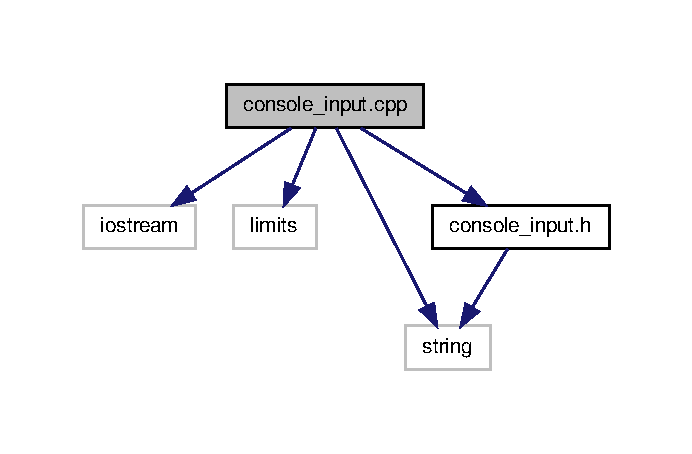
\includegraphics[width=332pt]{console__input_8cpp__incl}
\end{center}
\end{figure}
\subsection*{Functions}
\begin{DoxyCompactItemize}
\item 
double \hyperlink{console__input_8cpp_a8a9df77c5c4adba7ebadb77f3b3dc8ee}{read\-\_\-double} (double min, double max)
\item 
double \hyperlink{console__input_8cpp_a65f2421973540c10e5ae7d10177c566a}{read\-\_\-double} ()
\item 
double \hyperlink{console__input_8cpp_a46878a8594ba71f54911c572031d4614}{read\-\_\-double} (string text)
\item 
double \hyperlink{console__input_8cpp_aca43573be8fe10d4bfede3fc5bd0bd63}{read\-\_\-double} (string text, double min, double max)
\item 
long \hyperlink{console__input_8cpp_a710a686867142de265860584f4147592}{read\-\_\-long} (long min, long max)
\item 
long \hyperlink{console__input_8cpp_a347c616893b725a74f60ea1f7ee325d2}{read\-\_\-long} ()
\item 
long \hyperlink{console__input_8cpp_a9128c63513d87af5259597d8c9930476}{read\-\_\-long} (string text)
\item 
long \hyperlink{console__input_8cpp_a03ebbd2a45117ee03be4e9002210ab36}{read\-\_\-long} (string text, long min, long max)
\item 
int \hyperlink{console__input_8cpp_ad0ccfbb50d0e333ef8acfeab2b7d8071}{read\-\_\-int} (int min, int max)
\item 
int \hyperlink{console__input_8cpp_af310540093ee953c3018bc13bbde3da5}{read\-\_\-int} ()
\item 
int \hyperlink{console__input_8cpp_aaaf3786f6b4803f3120609011de4b0db}{read\-\_\-int} (string text)
\item 
int \hyperlink{console__input_8cpp_a4f8c1bb51d432116d3eda43db3340c8c}{read\-\_\-int} (string text, int min, int max)
\item 
bool \hyperlink{console__input_8cpp_a6bac3909a28fff2736a171022343380b}{read\-\_\-yes\-\_\-no} (string text)
\item 
string \hyperlink{console__input_8cpp_a44ccadd65be527f89bdcf6d27a3b1147}{read\-\_\-text} (string text)
\end{DoxyCompactItemize}


\subsection{Function Documentation}
\hypertarget{console__input_8cpp_a8a9df77c5c4adba7ebadb77f3b3dc8ee}{\index{console\-\_\-input.\-cpp@{console\-\_\-input.\-cpp}!read\-\_\-double@{read\-\_\-double}}
\index{read\-\_\-double@{read\-\_\-double}!console_input.cpp@{console\-\_\-input.\-cpp}}
\subsubsection[{read\-\_\-double}]{\setlength{\rightskip}{0pt plus 5cm}double read\-\_\-double (
\begin{DoxyParamCaption}
\item[{double}]{min, }
\item[{double}]{max}
\end{DoxyParamCaption}
)}}\label{console__input_8cpp_a8a9df77c5c4adba7ebadb77f3b3dc8ee}
Reads a double value in between a given interval from the console. When the entered value is not valid to the interval, the user gets prompted to reenter a valid.


\begin{DoxyParams}{Parameters}
{\em min} & lower bound of the interval. \\
\hline
{\em max} & top bound of the interval\\
\hline
\end{DoxyParams}
\begin{DoxyReturn}{Returns}
a double value in between min and max. 
\end{DoxyReturn}
\hypertarget{console__input_8cpp_a65f2421973540c10e5ae7d10177c566a}{\index{console\-\_\-input.\-cpp@{console\-\_\-input.\-cpp}!read\-\_\-double@{read\-\_\-double}}
\index{read\-\_\-double@{read\-\_\-double}!console_input.cpp@{console\-\_\-input.\-cpp}}
\subsubsection[{read\-\_\-double}]{\setlength{\rightskip}{0pt plus 5cm}double read\-\_\-double (
\begin{DoxyParamCaption}
{}
\end{DoxyParamCaption}
)}}\label{console__input_8cpp_a65f2421973540c10e5ae7d10177c566a}
Reads a double value from the console in between the whole range of double.

\begin{DoxyReturn}{Returns}
a valid double value. 
\end{DoxyReturn}


Here is the call graph for this function\-:\nopagebreak
\begin{figure}[H]
\begin{center}
\leavevmode
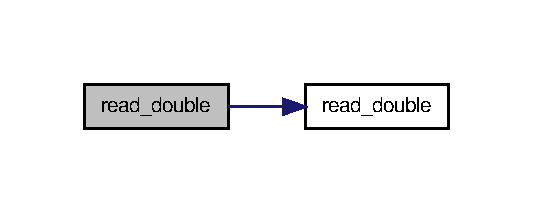
\includegraphics[width=256pt]{console__input_8cpp_a65f2421973540c10e5ae7d10177c566a_cgraph}
\end{center}
\end{figure}


\hypertarget{console__input_8cpp_a46878a8594ba71f54911c572031d4614}{\index{console\-\_\-input.\-cpp@{console\-\_\-input.\-cpp}!read\-\_\-double@{read\-\_\-double}}
\index{read\-\_\-double@{read\-\_\-double}!console_input.cpp@{console\-\_\-input.\-cpp}}
\subsubsection[{read\-\_\-double}]{\setlength{\rightskip}{0pt plus 5cm}double read\-\_\-double (
\begin{DoxyParamCaption}
\item[{string}]{text}
\end{DoxyParamCaption}
)}}\label{console__input_8cpp_a46878a8594ba71f54911c572031d4614}
Prints a text to the console and reads a double value from the console in between the whole range of double.


\begin{DoxyParams}{Parameters}
{\em text} & text to print to the console.\\
\hline
\end{DoxyParams}
\begin{DoxyReturn}{Returns}
a valid double value. 
\end{DoxyReturn}


Here is the call graph for this function\-:\nopagebreak
\begin{figure}[H]
\begin{center}
\leavevmode
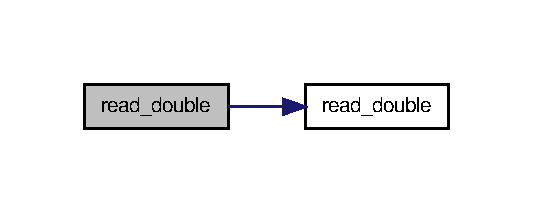
\includegraphics[width=256pt]{console__input_8cpp_a46878a8594ba71f54911c572031d4614_cgraph}
\end{center}
\end{figure}


\hypertarget{console__input_8cpp_aca43573be8fe10d4bfede3fc5bd0bd63}{\index{console\-\_\-input.\-cpp@{console\-\_\-input.\-cpp}!read\-\_\-double@{read\-\_\-double}}
\index{read\-\_\-double@{read\-\_\-double}!console_input.cpp@{console\-\_\-input.\-cpp}}
\subsubsection[{read\-\_\-double}]{\setlength{\rightskip}{0pt plus 5cm}double read\-\_\-double (
\begin{DoxyParamCaption}
\item[{string}]{text, }
\item[{double}]{min, }
\item[{double}]{max}
\end{DoxyParamCaption}
)}}\label{console__input_8cpp_aca43573be8fe10d4bfede3fc5bd0bd63}


Here is the call graph for this function\-:\nopagebreak
\begin{figure}[H]
\begin{center}
\leavevmode
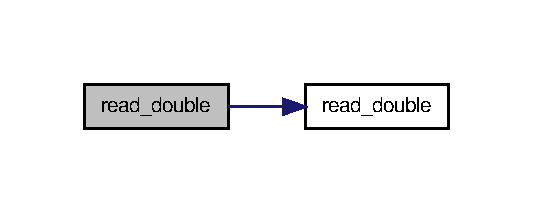
\includegraphics[width=256pt]{console__input_8cpp_aca43573be8fe10d4bfede3fc5bd0bd63_cgraph}
\end{center}
\end{figure}


\hypertarget{console__input_8cpp_ad0ccfbb50d0e333ef8acfeab2b7d8071}{\index{console\-\_\-input.\-cpp@{console\-\_\-input.\-cpp}!read\-\_\-int@{read\-\_\-int}}
\index{read\-\_\-int@{read\-\_\-int}!console_input.cpp@{console\-\_\-input.\-cpp}}
\subsubsection[{read\-\_\-int}]{\setlength{\rightskip}{0pt plus 5cm}int read\-\_\-int (
\begin{DoxyParamCaption}
\item[{int}]{min, }
\item[{int}]{max}
\end{DoxyParamCaption}
)}}\label{console__input_8cpp_ad0ccfbb50d0e333ef8acfeab2b7d8071}
Reads a integer value in between a given interval from the console. When the entered value is not valid to the interval, the user gets prompted to reenter a valid.


\begin{DoxyParams}{Parameters}
{\em min} & lower bound of the interval. \\
\hline
{\em max} & top bound of the interval\\
\hline
\end{DoxyParams}
\begin{DoxyReturn}{Returns}
a int value in between min and max. 
\end{DoxyReturn}


Here is the call graph for this function\-:\nopagebreak
\begin{figure}[H]
\begin{center}
\leavevmode
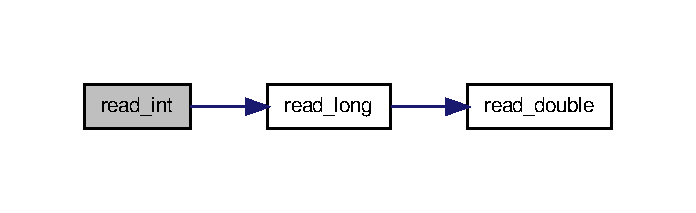
\includegraphics[width=334pt]{console__input_8cpp_ad0ccfbb50d0e333ef8acfeab2b7d8071_cgraph}
\end{center}
\end{figure}


\hypertarget{console__input_8cpp_af310540093ee953c3018bc13bbde3da5}{\index{console\-\_\-input.\-cpp@{console\-\_\-input.\-cpp}!read\-\_\-int@{read\-\_\-int}}
\index{read\-\_\-int@{read\-\_\-int}!console_input.cpp@{console\-\_\-input.\-cpp}}
\subsubsection[{read\-\_\-int}]{\setlength{\rightskip}{0pt plus 5cm}int read\-\_\-int (
\begin{DoxyParamCaption}
{}
\end{DoxyParamCaption}
)}}\label{console__input_8cpp_af310540093ee953c3018bc13bbde3da5}
Reads an integer value from the terminal in between the whole range of long.

\begin{DoxyReturn}{Returns}
a valid integer value. 
\end{DoxyReturn}


Here is the call graph for this function\-:\nopagebreak
\begin{figure}[H]
\begin{center}
\leavevmode
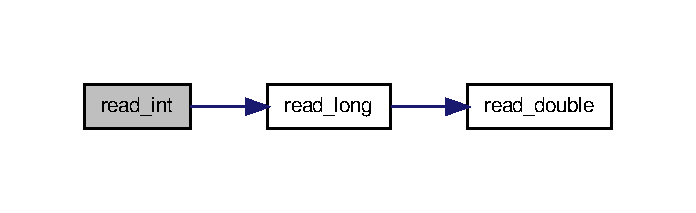
\includegraphics[width=334pt]{console__input_8cpp_af310540093ee953c3018bc13bbde3da5_cgraph}
\end{center}
\end{figure}


\hypertarget{console__input_8cpp_aaaf3786f6b4803f3120609011de4b0db}{\index{console\-\_\-input.\-cpp@{console\-\_\-input.\-cpp}!read\-\_\-int@{read\-\_\-int}}
\index{read\-\_\-int@{read\-\_\-int}!console_input.cpp@{console\-\_\-input.\-cpp}}
\subsubsection[{read\-\_\-int}]{\setlength{\rightskip}{0pt plus 5cm}int read\-\_\-int (
\begin{DoxyParamCaption}
\item[{string}]{text}
\end{DoxyParamCaption}
)}}\label{console__input_8cpp_aaaf3786f6b4803f3120609011de4b0db}
Prints a text to the console and reads a integer value from the console in between the whole range of integer.


\begin{DoxyParams}{Parameters}
{\em text} & text to print to the console.\\
\hline
\end{DoxyParams}
\begin{DoxyReturn}{Returns}
a valid integer value. 
\end{DoxyReturn}


Here is the call graph for this function\-:\nopagebreak
\begin{figure}[H]
\begin{center}
\leavevmode
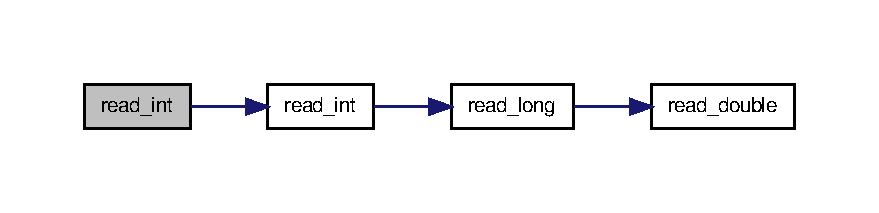
\includegraphics[width=350pt]{console__input_8cpp_aaaf3786f6b4803f3120609011de4b0db_cgraph}
\end{center}
\end{figure}


\hypertarget{console__input_8cpp_a4f8c1bb51d432116d3eda43db3340c8c}{\index{console\-\_\-input.\-cpp@{console\-\_\-input.\-cpp}!read\-\_\-int@{read\-\_\-int}}
\index{read\-\_\-int@{read\-\_\-int}!console_input.cpp@{console\-\_\-input.\-cpp}}
\subsubsection[{read\-\_\-int}]{\setlength{\rightskip}{0pt plus 5cm}int read\-\_\-int (
\begin{DoxyParamCaption}
\item[{string}]{text, }
\item[{int}]{min, }
\item[{int}]{max}
\end{DoxyParamCaption}
)}}\label{console__input_8cpp_a4f8c1bb51d432116d3eda43db3340c8c}
Prints a text to the console and reads a integer value in between a given interval from the console. When the value is not in between the interval, the user gets prompted to reeinter a valid value.


\begin{DoxyParams}{Parameters}
{\em text} & text to print to the console. \\
\hline
{\em min} & lower bound of the interval. \\
\hline
{\em max} & top bound of the interval.\\
\hline
\end{DoxyParams}
\begin{DoxyReturn}{Returns}
a integer value in between min and max. 
\end{DoxyReturn}


Here is the call graph for this function\-:\nopagebreak
\begin{figure}[H]
\begin{center}
\leavevmode
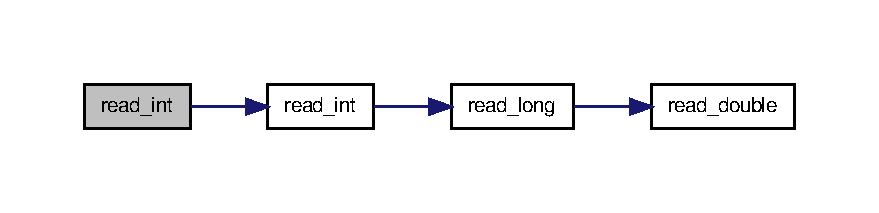
\includegraphics[width=350pt]{console__input_8cpp_a4f8c1bb51d432116d3eda43db3340c8c_cgraph}
\end{center}
\end{figure}


\hypertarget{console__input_8cpp_a710a686867142de265860584f4147592}{\index{console\-\_\-input.\-cpp@{console\-\_\-input.\-cpp}!read\-\_\-long@{read\-\_\-long}}
\index{read\-\_\-long@{read\-\_\-long}!console_input.cpp@{console\-\_\-input.\-cpp}}
\subsubsection[{read\-\_\-long}]{\setlength{\rightskip}{0pt plus 5cm}long read\-\_\-long (
\begin{DoxyParamCaption}
\item[{long}]{min, }
\item[{long}]{max}
\end{DoxyParamCaption}
)}}\label{console__input_8cpp_a710a686867142de265860584f4147592}
Reads a long value in between a given interval from the console. When the entered value is not valid to the interval, the user gets prompted to reenter a valid.


\begin{DoxyParams}{Parameters}
{\em min} & lower bound of the interval. \\
\hline
{\em max} & top bound of the interval\\
\hline
\end{DoxyParams}
\begin{DoxyReturn}{Returns}
a long value in between min and max. 
\end{DoxyReturn}


Here is the call graph for this function\-:\nopagebreak
\begin{figure}[H]
\begin{center}
\leavevmode
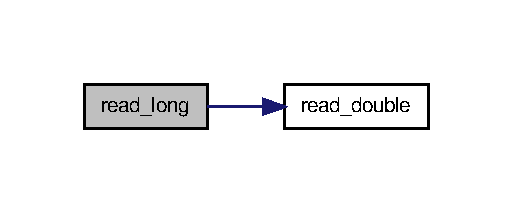
\includegraphics[width=246pt]{console__input_8cpp_a710a686867142de265860584f4147592_cgraph}
\end{center}
\end{figure}


\hypertarget{console__input_8cpp_a347c616893b725a74f60ea1f7ee325d2}{\index{console\-\_\-input.\-cpp@{console\-\_\-input.\-cpp}!read\-\_\-long@{read\-\_\-long}}
\index{read\-\_\-long@{read\-\_\-long}!console_input.cpp@{console\-\_\-input.\-cpp}}
\subsubsection[{read\-\_\-long}]{\setlength{\rightskip}{0pt plus 5cm}long read\-\_\-long (
\begin{DoxyParamCaption}
{}
\end{DoxyParamCaption}
)}}\label{console__input_8cpp_a347c616893b725a74f60ea1f7ee325d2}
Reads a long value from the terminal in between the whole range of long.

\begin{DoxyReturn}{Returns}
a valid long value. 
\end{DoxyReturn}


Here is the call graph for this function\-:\nopagebreak
\begin{figure}[H]
\begin{center}
\leavevmode
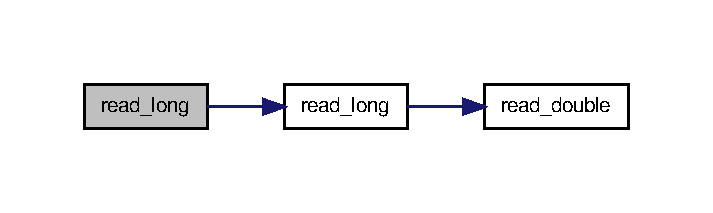
\includegraphics[width=342pt]{console__input_8cpp_a347c616893b725a74f60ea1f7ee325d2_cgraph}
\end{center}
\end{figure}


\hypertarget{console__input_8cpp_a9128c63513d87af5259597d8c9930476}{\index{console\-\_\-input.\-cpp@{console\-\_\-input.\-cpp}!read\-\_\-long@{read\-\_\-long}}
\index{read\-\_\-long@{read\-\_\-long}!console_input.cpp@{console\-\_\-input.\-cpp}}
\subsubsection[{read\-\_\-long}]{\setlength{\rightskip}{0pt plus 5cm}long read\-\_\-long (
\begin{DoxyParamCaption}
\item[{string}]{text}
\end{DoxyParamCaption}
)}}\label{console__input_8cpp_a9128c63513d87af5259597d8c9930476}
Prints a text to the console and reads a long value from the console in between the whole range of long.


\begin{DoxyParams}{Parameters}
{\em text} & text to print to the console.\\
\hline
\end{DoxyParams}
\begin{DoxyReturn}{Returns}
a valid long value. 
\end{DoxyReturn}


Here is the call graph for this function\-:\nopagebreak
\begin{figure}[H]
\begin{center}
\leavevmode
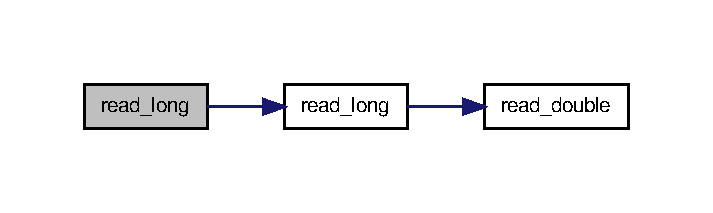
\includegraphics[width=342pt]{console__input_8cpp_a9128c63513d87af5259597d8c9930476_cgraph}
\end{center}
\end{figure}


\hypertarget{console__input_8cpp_a03ebbd2a45117ee03be4e9002210ab36}{\index{console\-\_\-input.\-cpp@{console\-\_\-input.\-cpp}!read\-\_\-long@{read\-\_\-long}}
\index{read\-\_\-long@{read\-\_\-long}!console_input.cpp@{console\-\_\-input.\-cpp}}
\subsubsection[{read\-\_\-long}]{\setlength{\rightskip}{0pt plus 5cm}long read\-\_\-long (
\begin{DoxyParamCaption}
\item[{string}]{text, }
\item[{long}]{min, }
\item[{long}]{max}
\end{DoxyParamCaption}
)}}\label{console__input_8cpp_a03ebbd2a45117ee03be4e9002210ab36}
Prints a text to the console and reads a long value in between a given interval from the console. When the value is not in between the interval, the user gets prompted to reeinter a valid value.


\begin{DoxyParams}{Parameters}
{\em text} & text to print to the console. \\
\hline
{\em min} & lower bound of the interval. \\
\hline
{\em max} & top bound of the interval.\\
\hline
\end{DoxyParams}
\begin{DoxyReturn}{Returns}
a long value in between min and max. 
\end{DoxyReturn}


Here is the call graph for this function\-:\nopagebreak
\begin{figure}[H]
\begin{center}
\leavevmode
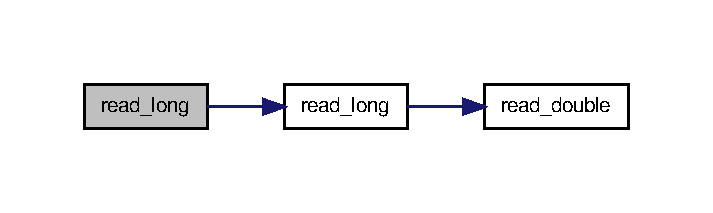
\includegraphics[width=342pt]{console__input_8cpp_a03ebbd2a45117ee03be4e9002210ab36_cgraph}
\end{center}
\end{figure}


\hypertarget{console__input_8cpp_a44ccadd65be527f89bdcf6d27a3b1147}{\index{console\-\_\-input.\-cpp@{console\-\_\-input.\-cpp}!read\-\_\-text@{read\-\_\-text}}
\index{read\-\_\-text@{read\-\_\-text}!console_input.cpp@{console\-\_\-input.\-cpp}}
\subsubsection[{read\-\_\-text}]{\setlength{\rightskip}{0pt plus 5cm}string read\-\_\-text (
\begin{DoxyParamCaption}
\item[{string}]{text}
\end{DoxyParamCaption}
)}}\label{console__input_8cpp_a44ccadd65be527f89bdcf6d27a3b1147}
\hypertarget{console__input_8cpp_a6bac3909a28fff2736a171022343380b}{\index{console\-\_\-input.\-cpp@{console\-\_\-input.\-cpp}!read\-\_\-yes\-\_\-no@{read\-\_\-yes\-\_\-no}}
\index{read\-\_\-yes\-\_\-no@{read\-\_\-yes\-\_\-no}!console_input.cpp@{console\-\_\-input.\-cpp}}
\subsubsection[{read\-\_\-yes\-\_\-no}]{\setlength{\rightskip}{0pt plus 5cm}bool read\-\_\-yes\-\_\-no (
\begin{DoxyParamCaption}
\item[{string}]{text}
\end{DoxyParamCaption}
)}}\label{console__input_8cpp_a6bac3909a28fff2736a171022343380b}

\hypertarget{console__input_8h}{\section{console\-\_\-input.\-h File Reference}
\label{console__input_8h}\index{console\-\_\-input.\-h@{console\-\_\-input.\-h}}
}
{\ttfamily \#include $<$string$>$}\\*
Include dependency graph for console\-\_\-input.\-h\-:\nopagebreak
\begin{figure}[H]
\begin{center}
\leavevmode
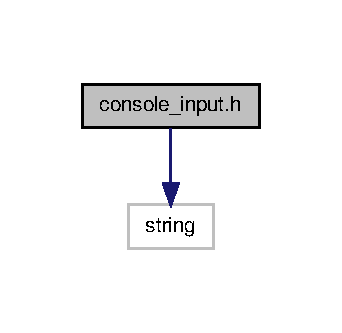
\includegraphics[width=164pt]{console__input_8h__incl}
\end{center}
\end{figure}
This graph shows which files directly or indirectly include this file\-:\nopagebreak
\begin{figure}[H]
\begin{center}
\leavevmode
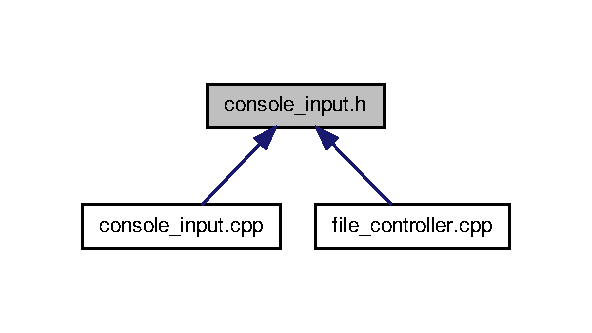
\includegraphics[width=264pt]{console__input_8h__dep__incl}
\end{center}
\end{figure}
\subsection*{Functions}
\begin{DoxyCompactItemize}
\item 
double \hyperlink{console__input_8h_a8a9df77c5c4adba7ebadb77f3b3dc8ee}{read\-\_\-double} (double min, double max)
\item 
double \hyperlink{console__input_8h_a46878a8594ba71f54911c572031d4614}{read\-\_\-double} (string text)
\item 
double \hyperlink{console__input_8h_aca43573be8fe10d4bfede3fc5bd0bd63}{read\-\_\-double} (string text, double min, double max)
\item 
double \hyperlink{console__input_8h_a65f2421973540c10e5ae7d10177c566a}{read\-\_\-double} ()
\item 
void \hyperlink{console__input_8h_afc6e4adf69aec96a5eae4249fbbc7201}{read\-\_\-enter} ()
\item 
long \hyperlink{console__input_8h_a03ebbd2a45117ee03be4e9002210ab36}{read\-\_\-long} (string text, long min, long max)
\item 
long \hyperlink{console__input_8h_a710a686867142de265860584f4147592}{read\-\_\-long} (long min, long max)
\item 
long \hyperlink{console__input_8h_a9128c63513d87af5259597d8c9930476}{read\-\_\-long} (string text)
\item 
long \hyperlink{console__input_8h_a347c616893b725a74f60ea1f7ee325d2}{read\-\_\-long} ()
\item 
int \hyperlink{console__input_8h_a4f8c1bb51d432116d3eda43db3340c8c}{read\-\_\-int} (string text, int min, int max)
\item 
int \hyperlink{console__input_8h_ad0ccfbb50d0e333ef8acfeab2b7d8071}{read\-\_\-int} (int min, int max)
\item 
int \hyperlink{console__input_8h_aaaf3786f6b4803f3120609011de4b0db}{read\-\_\-int} (string text)
\item 
int \hyperlink{console__input_8h_af310540093ee953c3018bc13bbde3da5}{read\-\_\-int} ()
\item 
bool \hyperlink{console__input_8h_a6bac3909a28fff2736a171022343380b}{read\-\_\-yes\-\_\-no} (string text)
\item 
string \hyperlink{console__input_8h_a44ccadd65be527f89bdcf6d27a3b1147}{read\-\_\-text} (string text)
\end{DoxyCompactItemize}


\subsection{Function Documentation}
\hypertarget{console__input_8h_a8a9df77c5c4adba7ebadb77f3b3dc8ee}{\index{console\-\_\-input.\-h@{console\-\_\-input.\-h}!read\-\_\-double@{read\-\_\-double}}
\index{read\-\_\-double@{read\-\_\-double}!console_input.h@{console\-\_\-input.\-h}}
\subsubsection[{read\-\_\-double}]{\setlength{\rightskip}{0pt plus 5cm}double read\-\_\-double (
\begin{DoxyParamCaption}
\item[{double}]{min, }
\item[{double}]{max}
\end{DoxyParamCaption}
)}}\label{console__input_8h_a8a9df77c5c4adba7ebadb77f3b3dc8ee}
Reads a double value in between a given interval from the console. When the entered value is not valid to the interval, the user gets prompted to reenter a valid.


\begin{DoxyParams}{Parameters}
{\em min} & lower bound of the interval. \\
\hline
{\em max} & top bound of the interval\\
\hline
\end{DoxyParams}
\begin{DoxyReturn}{Returns}
a double value in between min and max. 
\end{DoxyReturn}
\hypertarget{console__input_8h_a46878a8594ba71f54911c572031d4614}{\index{console\-\_\-input.\-h@{console\-\_\-input.\-h}!read\-\_\-double@{read\-\_\-double}}
\index{read\-\_\-double@{read\-\_\-double}!console_input.h@{console\-\_\-input.\-h}}
\subsubsection[{read\-\_\-double}]{\setlength{\rightskip}{0pt plus 5cm}double read\-\_\-double (
\begin{DoxyParamCaption}
\item[{string}]{text}
\end{DoxyParamCaption}
)}}\label{console__input_8h_a46878a8594ba71f54911c572031d4614}
Prints a text to the console and reads a double value from the console in between the whole range of double.


\begin{DoxyParams}{Parameters}
{\em text} & text to print to the console.\\
\hline
\end{DoxyParams}
\begin{DoxyReturn}{Returns}
a valid double value. 
\end{DoxyReturn}


Here is the call graph for this function\-:\nopagebreak
\begin{figure}[H]
\begin{center}
\leavevmode
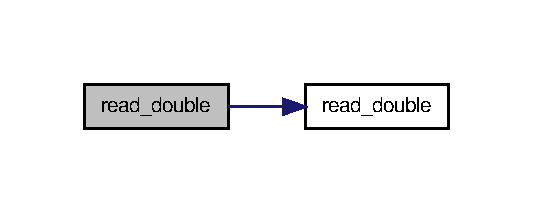
\includegraphics[width=256pt]{console__input_8h_a46878a8594ba71f54911c572031d4614_cgraph}
\end{center}
\end{figure}


\hypertarget{console__input_8h_aca43573be8fe10d4bfede3fc5bd0bd63}{\index{console\-\_\-input.\-h@{console\-\_\-input.\-h}!read\-\_\-double@{read\-\_\-double}}
\index{read\-\_\-double@{read\-\_\-double}!console_input.h@{console\-\_\-input.\-h}}
\subsubsection[{read\-\_\-double}]{\setlength{\rightskip}{0pt plus 5cm}double read\-\_\-double (
\begin{DoxyParamCaption}
\item[{string}]{text, }
\item[{double}]{min, }
\item[{double}]{max}
\end{DoxyParamCaption}
)}}\label{console__input_8h_aca43573be8fe10d4bfede3fc5bd0bd63}


Here is the call graph for this function\-:\nopagebreak
\begin{figure}[H]
\begin{center}
\leavevmode
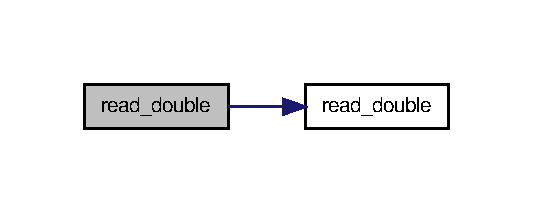
\includegraphics[width=256pt]{console__input_8h_aca43573be8fe10d4bfede3fc5bd0bd63_cgraph}
\end{center}
\end{figure}


\hypertarget{console__input_8h_a65f2421973540c10e5ae7d10177c566a}{\index{console\-\_\-input.\-h@{console\-\_\-input.\-h}!read\-\_\-double@{read\-\_\-double}}
\index{read\-\_\-double@{read\-\_\-double}!console_input.h@{console\-\_\-input.\-h}}
\subsubsection[{read\-\_\-double}]{\setlength{\rightskip}{0pt plus 5cm}double read\-\_\-double (
\begin{DoxyParamCaption}
{}
\end{DoxyParamCaption}
)}}\label{console__input_8h_a65f2421973540c10e5ae7d10177c566a}
Reads a double value from the console in between the whole range of double.

\begin{DoxyReturn}{Returns}
a valid double value. 
\end{DoxyReturn}


Here is the call graph for this function\-:\nopagebreak
\begin{figure}[H]
\begin{center}
\leavevmode
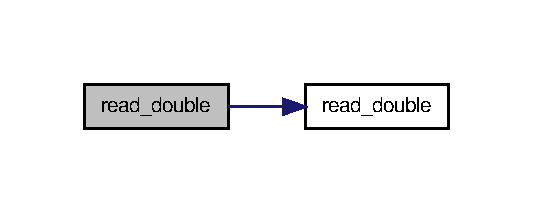
\includegraphics[width=256pt]{console__input_8h_a65f2421973540c10e5ae7d10177c566a_cgraph}
\end{center}
\end{figure}


\hypertarget{console__input_8h_afc6e4adf69aec96a5eae4249fbbc7201}{\index{console\-\_\-input.\-h@{console\-\_\-input.\-h}!read\-\_\-enter@{read\-\_\-enter}}
\index{read\-\_\-enter@{read\-\_\-enter}!console_input.h@{console\-\_\-input.\-h}}
\subsubsection[{read\-\_\-enter}]{\setlength{\rightskip}{0pt plus 5cm}void read\-\_\-enter (
\begin{DoxyParamCaption}
{}
\end{DoxyParamCaption}
)}}\label{console__input_8h_afc6e4adf69aec96a5eae4249fbbc7201}
\hypertarget{console__input_8h_a4f8c1bb51d432116d3eda43db3340c8c}{\index{console\-\_\-input.\-h@{console\-\_\-input.\-h}!read\-\_\-int@{read\-\_\-int}}
\index{read\-\_\-int@{read\-\_\-int}!console_input.h@{console\-\_\-input.\-h}}
\subsubsection[{read\-\_\-int}]{\setlength{\rightskip}{0pt plus 5cm}int read\-\_\-int (
\begin{DoxyParamCaption}
\item[{string}]{text, }
\item[{int}]{min, }
\item[{int}]{max}
\end{DoxyParamCaption}
)}}\label{console__input_8h_a4f8c1bb51d432116d3eda43db3340c8c}
Prints a text to the console and reads a integer value in between a given interval from the console. When the value is not in between the interval, the user gets prompted to reeinter a valid value.


\begin{DoxyParams}{Parameters}
{\em text} & text to print to the console. \\
\hline
{\em min} & lower bound of the interval. \\
\hline
{\em max} & top bound of the interval.\\
\hline
\end{DoxyParams}
\begin{DoxyReturn}{Returns}
a integer value in between min and max. 
\end{DoxyReturn}


Here is the call graph for this function\-:\nopagebreak
\begin{figure}[H]
\begin{center}
\leavevmode
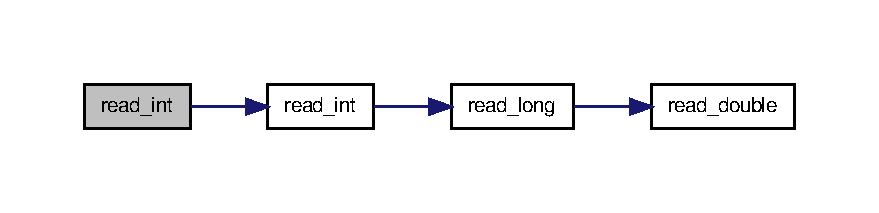
\includegraphics[width=350pt]{console__input_8h_a4f8c1bb51d432116d3eda43db3340c8c_cgraph}
\end{center}
\end{figure}


\hypertarget{console__input_8h_ad0ccfbb50d0e333ef8acfeab2b7d8071}{\index{console\-\_\-input.\-h@{console\-\_\-input.\-h}!read\-\_\-int@{read\-\_\-int}}
\index{read\-\_\-int@{read\-\_\-int}!console_input.h@{console\-\_\-input.\-h}}
\subsubsection[{read\-\_\-int}]{\setlength{\rightskip}{0pt plus 5cm}int read\-\_\-int (
\begin{DoxyParamCaption}
\item[{int}]{min, }
\item[{int}]{max}
\end{DoxyParamCaption}
)}}\label{console__input_8h_ad0ccfbb50d0e333ef8acfeab2b7d8071}
Reads a integer value in between a given interval from the console. When the entered value is not valid to the interval, the user gets prompted to reenter a valid.


\begin{DoxyParams}{Parameters}
{\em min} & lower bound of the interval. \\
\hline
{\em max} & top bound of the interval\\
\hline
\end{DoxyParams}
\begin{DoxyReturn}{Returns}
a int value in between min and max. 
\end{DoxyReturn}


Here is the call graph for this function\-:\nopagebreak
\begin{figure}[H]
\begin{center}
\leavevmode
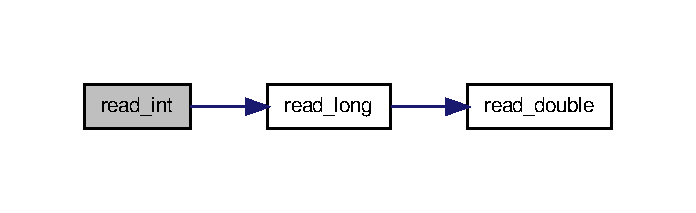
\includegraphics[width=334pt]{console__input_8h_ad0ccfbb50d0e333ef8acfeab2b7d8071_cgraph}
\end{center}
\end{figure}


\hypertarget{console__input_8h_aaaf3786f6b4803f3120609011de4b0db}{\index{console\-\_\-input.\-h@{console\-\_\-input.\-h}!read\-\_\-int@{read\-\_\-int}}
\index{read\-\_\-int@{read\-\_\-int}!console_input.h@{console\-\_\-input.\-h}}
\subsubsection[{read\-\_\-int}]{\setlength{\rightskip}{0pt plus 5cm}int read\-\_\-int (
\begin{DoxyParamCaption}
\item[{string}]{text}
\end{DoxyParamCaption}
)}}\label{console__input_8h_aaaf3786f6b4803f3120609011de4b0db}
Prints a text to the console and reads a integer value from the console in between the whole range of integer.


\begin{DoxyParams}{Parameters}
{\em text} & text to print to the console.\\
\hline
\end{DoxyParams}
\begin{DoxyReturn}{Returns}
a valid integer value. 
\end{DoxyReturn}


Here is the call graph for this function\-:\nopagebreak
\begin{figure}[H]
\begin{center}
\leavevmode
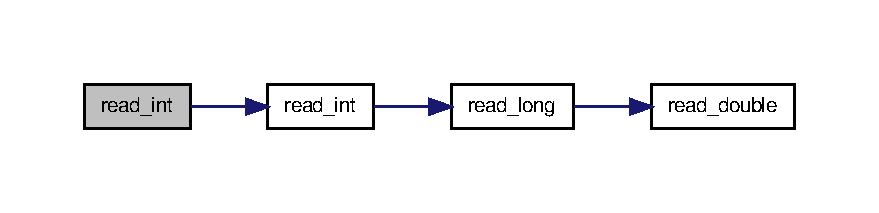
\includegraphics[width=350pt]{console__input_8h_aaaf3786f6b4803f3120609011de4b0db_cgraph}
\end{center}
\end{figure}


\hypertarget{console__input_8h_af310540093ee953c3018bc13bbde3da5}{\index{console\-\_\-input.\-h@{console\-\_\-input.\-h}!read\-\_\-int@{read\-\_\-int}}
\index{read\-\_\-int@{read\-\_\-int}!console_input.h@{console\-\_\-input.\-h}}
\subsubsection[{read\-\_\-int}]{\setlength{\rightskip}{0pt plus 5cm}int read\-\_\-int (
\begin{DoxyParamCaption}
{}
\end{DoxyParamCaption}
)}}\label{console__input_8h_af310540093ee953c3018bc13bbde3da5}
Reads an integer value from the terminal in between the whole range of long.

\begin{DoxyReturn}{Returns}
a valid integer value. 
\end{DoxyReturn}


Here is the call graph for this function\-:\nopagebreak
\begin{figure}[H]
\begin{center}
\leavevmode
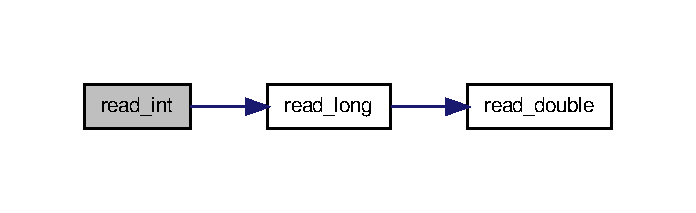
\includegraphics[width=334pt]{console__input_8h_af310540093ee953c3018bc13bbde3da5_cgraph}
\end{center}
\end{figure}


\hypertarget{console__input_8h_a03ebbd2a45117ee03be4e9002210ab36}{\index{console\-\_\-input.\-h@{console\-\_\-input.\-h}!read\-\_\-long@{read\-\_\-long}}
\index{read\-\_\-long@{read\-\_\-long}!console_input.h@{console\-\_\-input.\-h}}
\subsubsection[{read\-\_\-long}]{\setlength{\rightskip}{0pt plus 5cm}long read\-\_\-long (
\begin{DoxyParamCaption}
\item[{string}]{text, }
\item[{long}]{min, }
\item[{long}]{max}
\end{DoxyParamCaption}
)}}\label{console__input_8h_a03ebbd2a45117ee03be4e9002210ab36}
Prints a text to the console and reads a long value in between a given interval from the console. When the value is not in between the interval, the user gets prompted to reeinter a valid value.


\begin{DoxyParams}{Parameters}
{\em text} & text to print to the console. \\
\hline
{\em min} & lower bound of the interval. \\
\hline
{\em max} & top bound of the interval.\\
\hline
\end{DoxyParams}
\begin{DoxyReturn}{Returns}
a long value in between min and max. 
\end{DoxyReturn}


Here is the call graph for this function\-:\nopagebreak
\begin{figure}[H]
\begin{center}
\leavevmode
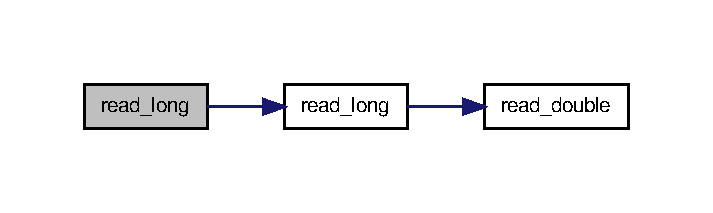
\includegraphics[width=342pt]{console__input_8h_a03ebbd2a45117ee03be4e9002210ab36_cgraph}
\end{center}
\end{figure}


\hypertarget{console__input_8h_a710a686867142de265860584f4147592}{\index{console\-\_\-input.\-h@{console\-\_\-input.\-h}!read\-\_\-long@{read\-\_\-long}}
\index{read\-\_\-long@{read\-\_\-long}!console_input.h@{console\-\_\-input.\-h}}
\subsubsection[{read\-\_\-long}]{\setlength{\rightskip}{0pt plus 5cm}long read\-\_\-long (
\begin{DoxyParamCaption}
\item[{long}]{min, }
\item[{long}]{max}
\end{DoxyParamCaption}
)}}\label{console__input_8h_a710a686867142de265860584f4147592}
Reads a long value in between a given interval from the console. When the entered value is not valid to the interval, the user gets prompted to reenter a valid.


\begin{DoxyParams}{Parameters}
{\em min} & lower bound of the interval. \\
\hline
{\em max} & top bound of the interval\\
\hline
\end{DoxyParams}
\begin{DoxyReturn}{Returns}
a long value in between min and max. 
\end{DoxyReturn}


Here is the call graph for this function\-:\nopagebreak
\begin{figure}[H]
\begin{center}
\leavevmode
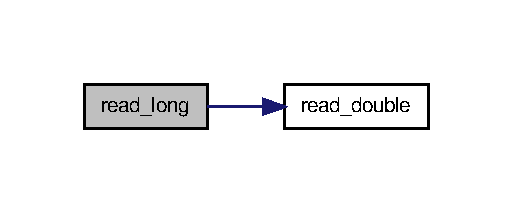
\includegraphics[width=246pt]{console__input_8h_a710a686867142de265860584f4147592_cgraph}
\end{center}
\end{figure}


\hypertarget{console__input_8h_a9128c63513d87af5259597d8c9930476}{\index{console\-\_\-input.\-h@{console\-\_\-input.\-h}!read\-\_\-long@{read\-\_\-long}}
\index{read\-\_\-long@{read\-\_\-long}!console_input.h@{console\-\_\-input.\-h}}
\subsubsection[{read\-\_\-long}]{\setlength{\rightskip}{0pt plus 5cm}long read\-\_\-long (
\begin{DoxyParamCaption}
\item[{string}]{text}
\end{DoxyParamCaption}
)}}\label{console__input_8h_a9128c63513d87af5259597d8c9930476}
Prints a text to the console and reads a long value from the console in between the whole range of long.


\begin{DoxyParams}{Parameters}
{\em text} & text to print to the console.\\
\hline
\end{DoxyParams}
\begin{DoxyReturn}{Returns}
a valid long value. 
\end{DoxyReturn}


Here is the call graph for this function\-:\nopagebreak
\begin{figure}[H]
\begin{center}
\leavevmode
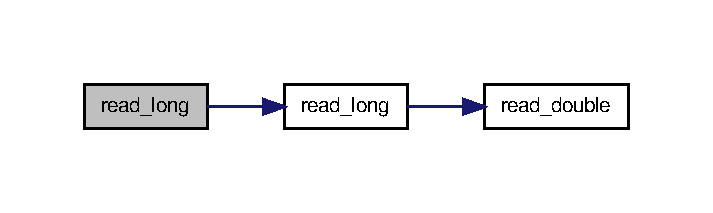
\includegraphics[width=342pt]{console__input_8h_a9128c63513d87af5259597d8c9930476_cgraph}
\end{center}
\end{figure}


\hypertarget{console__input_8h_a347c616893b725a74f60ea1f7ee325d2}{\index{console\-\_\-input.\-h@{console\-\_\-input.\-h}!read\-\_\-long@{read\-\_\-long}}
\index{read\-\_\-long@{read\-\_\-long}!console_input.h@{console\-\_\-input.\-h}}
\subsubsection[{read\-\_\-long}]{\setlength{\rightskip}{0pt plus 5cm}long read\-\_\-long (
\begin{DoxyParamCaption}
{}
\end{DoxyParamCaption}
)}}\label{console__input_8h_a347c616893b725a74f60ea1f7ee325d2}
Reads a long value from the terminal in between the whole range of long.

\begin{DoxyReturn}{Returns}
a valid long value. 
\end{DoxyReturn}


Here is the call graph for this function\-:\nopagebreak
\begin{figure}[H]
\begin{center}
\leavevmode
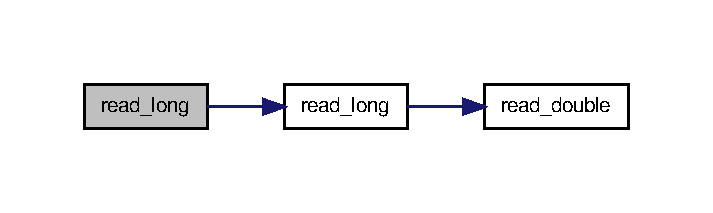
\includegraphics[width=342pt]{console__input_8h_a347c616893b725a74f60ea1f7ee325d2_cgraph}
\end{center}
\end{figure}


\hypertarget{console__input_8h_a44ccadd65be527f89bdcf6d27a3b1147}{\index{console\-\_\-input.\-h@{console\-\_\-input.\-h}!read\-\_\-text@{read\-\_\-text}}
\index{read\-\_\-text@{read\-\_\-text}!console_input.h@{console\-\_\-input.\-h}}
\subsubsection[{read\-\_\-text}]{\setlength{\rightskip}{0pt plus 5cm}string read\-\_\-text (
\begin{DoxyParamCaption}
\item[{string}]{text}
\end{DoxyParamCaption}
)}}\label{console__input_8h_a44ccadd65be527f89bdcf6d27a3b1147}
\hypertarget{console__input_8h_a6bac3909a28fff2736a171022343380b}{\index{console\-\_\-input.\-h@{console\-\_\-input.\-h}!read\-\_\-yes\-\_\-no@{read\-\_\-yes\-\_\-no}}
\index{read\-\_\-yes\-\_\-no@{read\-\_\-yes\-\_\-no}!console_input.h@{console\-\_\-input.\-h}}
\subsubsection[{read\-\_\-yes\-\_\-no}]{\setlength{\rightskip}{0pt plus 5cm}bool read\-\_\-yes\-\_\-no (
\begin{DoxyParamCaption}
\item[{string}]{text}
\end{DoxyParamCaption}
)}}\label{console__input_8h_a6bac3909a28fff2736a171022343380b}

\hypertarget{file__controller_8cpp}{\section{file\-\_\-controller.\-cpp File Reference}
\label{file__controller_8cpp}\index{file\-\_\-controller.\-cpp@{file\-\_\-controller.\-cpp}}
}
{\ttfamily \#include $<$iostream$>$}\\*
{\ttfamily \#include $<$string$>$}\\*
{\ttfamily \#include $<$fstream$>$}\\*
{\ttfamily \#include \char`\"{}console\-\_\-input.\-h\char`\"{}}\\*
{\ttfamily \#include \char`\"{}file\-\_\-controller.\-h\char`\"{}}\\*
Include dependency graph for file\-\_\-controller.\-cpp\-:\nopagebreak
\begin{figure}[H]
\begin{center}
\leavevmode
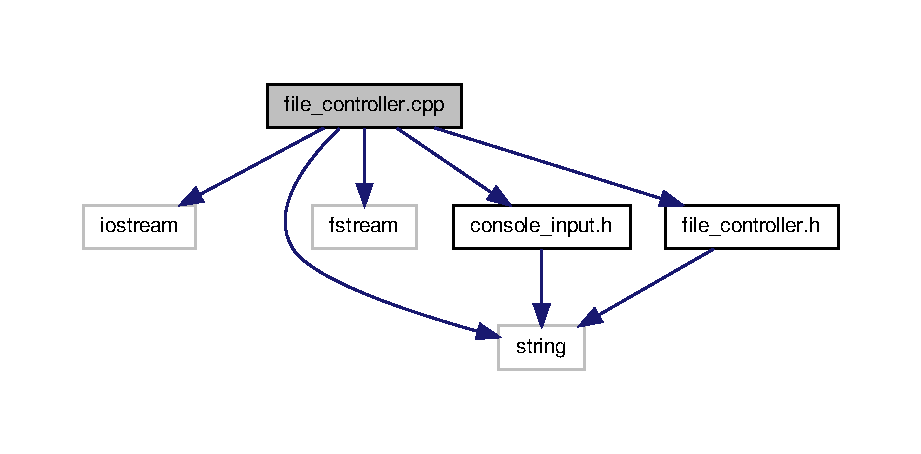
\includegraphics[width=350pt]{file__controller_8cpp__incl}
\end{center}
\end{figure}
\subsection*{Functions}
\begin{DoxyCompactItemize}
\item 
void \hyperlink{file__controller_8cpp_a8600a74cc7b9657c803885b9f6844fe7}{write\-\_\-to\-\_\-file} (string filename, string text, bool secure)
\item 
void \hyperlink{file__controller_8cpp_a90ee1f4929750a48a0e201f8923a2449}{write\-\_\-to\-\_\-file} (string text)
\item 
bool \hyperlink{file__controller_8cpp_acde73c899ec0618eeb8ae54b0a823f39}{file\-\_\-exists} (const std\-::string \&filename)
\item 
string \hyperlink{file__controller_8cpp_a5b269a712c2a290dd75694ab5ed3cb18}{read\-\_\-secure\-\_\-filename} ()
\end{DoxyCompactItemize}


\subsection{Function Documentation}
\hypertarget{file__controller_8cpp_acde73c899ec0618eeb8ae54b0a823f39}{\index{file\-\_\-controller.\-cpp@{file\-\_\-controller.\-cpp}!file\-\_\-exists@{file\-\_\-exists}}
\index{file\-\_\-exists@{file\-\_\-exists}!file_controller.cpp@{file\-\_\-controller.\-cpp}}
\subsubsection[{file\-\_\-exists}]{\setlength{\rightskip}{0pt plus 5cm}bool file\-\_\-exists (
\begin{DoxyParamCaption}
\item[{const std\-::string \&}]{filename}
\end{DoxyParamCaption}
)}}\label{file__controller_8cpp_acde73c899ec0618eeb8ae54b0a823f39}
Checks if a file already exists by its name.


\begin{DoxyParams}{Parameters}
{\em filename} & Filename to check for existence.\\
\hline
\end{DoxyParams}
\begin{DoxyReturn}{Returns}
true when the file exists. false when the file don't exists. 
\end{DoxyReturn}
\hypertarget{file__controller_8cpp_a5b269a712c2a290dd75694ab5ed3cb18}{\index{file\-\_\-controller.\-cpp@{file\-\_\-controller.\-cpp}!read\-\_\-secure\-\_\-filename@{read\-\_\-secure\-\_\-filename}}
\index{read\-\_\-secure\-\_\-filename@{read\-\_\-secure\-\_\-filename}!file_controller.cpp@{file\-\_\-controller.\-cpp}}
\subsubsection[{read\-\_\-secure\-\_\-filename}]{\setlength{\rightskip}{0pt plus 5cm}string read\-\_\-secure\-\_\-filename (
\begin{DoxyParamCaption}
{}
\end{DoxyParamCaption}
)}}\label{file__controller_8cpp_a5b269a712c2a290dd75694ab5ed3cb18}
Promts the user to enter a filename. The filename gets checked for existance. When there is already an existing file for the enterd filename, the user gets promted to override or reenter e new name.

\begin{DoxyReturn}{Returns}
a filename of a new file or of an existing file which can be overwritten. 
\end{DoxyReturn}


Here is the call graph for this function\-:\nopagebreak
\begin{figure}[H]
\begin{center}
\leavevmode
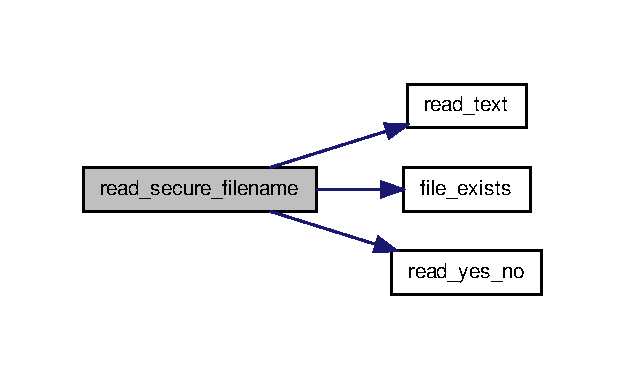
\includegraphics[width=300pt]{file__controller_8cpp_a5b269a712c2a290dd75694ab5ed3cb18_cgraph}
\end{center}
\end{figure}


\hypertarget{file__controller_8cpp_a8600a74cc7b9657c803885b9f6844fe7}{\index{file\-\_\-controller.\-cpp@{file\-\_\-controller.\-cpp}!write\-\_\-to\-\_\-file@{write\-\_\-to\-\_\-file}}
\index{write\-\_\-to\-\_\-file@{write\-\_\-to\-\_\-file}!file_controller.cpp@{file\-\_\-controller.\-cpp}}
\subsubsection[{write\-\_\-to\-\_\-file}]{\setlength{\rightskip}{0pt plus 5cm}void write\-\_\-to\-\_\-file (
\begin{DoxyParamCaption}
\item[{string}]{filename, }
\item[{string}]{text, }
\item[{bool}]{secure}
\end{DoxyParamCaption}
)}}\label{file__controller_8cpp_a8600a74cc7b9657c803885b9f6844fe7}
Writes given text into a file with the given filename.


\begin{DoxyParams}{Parameters}
{\em filename} & Name of the file to wirte. \\
\hline
{\em text} & Text to write into the file. \\
\hline
\end{DoxyParams}


Here is the call graph for this function\-:\nopagebreak
\begin{figure}[H]
\begin{center}
\leavevmode
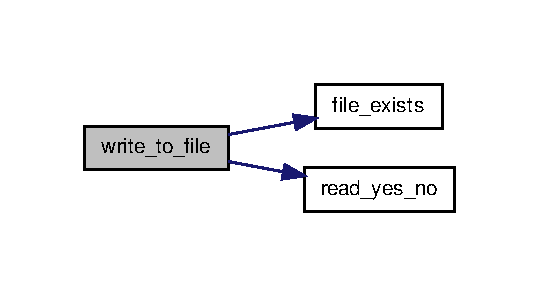
\includegraphics[width=258pt]{file__controller_8cpp_a8600a74cc7b9657c803885b9f6844fe7_cgraph}
\end{center}
\end{figure}


\hypertarget{file__controller_8cpp_a90ee1f4929750a48a0e201f8923a2449}{\index{file\-\_\-controller.\-cpp@{file\-\_\-controller.\-cpp}!write\-\_\-to\-\_\-file@{write\-\_\-to\-\_\-file}}
\index{write\-\_\-to\-\_\-file@{write\-\_\-to\-\_\-file}!file_controller.cpp@{file\-\_\-controller.\-cpp}}
\subsubsection[{write\-\_\-to\-\_\-file}]{\setlength{\rightskip}{0pt plus 5cm}void write\-\_\-to\-\_\-file (
\begin{DoxyParamCaption}
\item[{string}]{text}
\end{DoxyParamCaption}
)}}\label{file__controller_8cpp_a90ee1f4929750a48a0e201f8923a2449}
Writes a given text into a file. The name of the file has to be entered by the user. When the file already exists. The user gets prompted to overwrite or entering a new name.


\begin{DoxyParams}{Parameters}
{\em text} & Text to write into the file. \\
\hline
\end{DoxyParams}


Here is the call graph for this function\-:\nopagebreak
\begin{figure}[H]
\begin{center}
\leavevmode
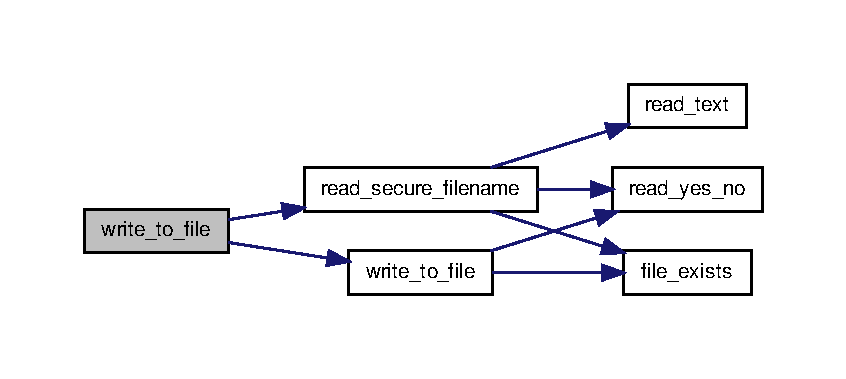
\includegraphics[width=350pt]{file__controller_8cpp_a90ee1f4929750a48a0e201f8923a2449_cgraph}
\end{center}
\end{figure}



\hypertarget{file__controller_8h}{\section{file\-\_\-controller.\-h File Reference}
\label{file__controller_8h}\index{file\-\_\-controller.\-h@{file\-\_\-controller.\-h}}
}
{\ttfamily \#include $<$string$>$}\\*
Include dependency graph for file\-\_\-controller.\-h\-:\nopagebreak
\begin{figure}[H]
\begin{center}
\leavevmode
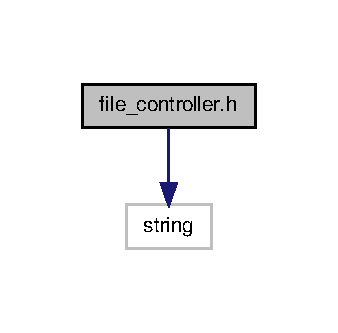
\includegraphics[width=162pt]{file__controller_8h__incl}
\end{center}
\end{figure}
This graph shows which files directly or indirectly include this file\-:\nopagebreak
\begin{figure}[H]
\begin{center}
\leavevmode
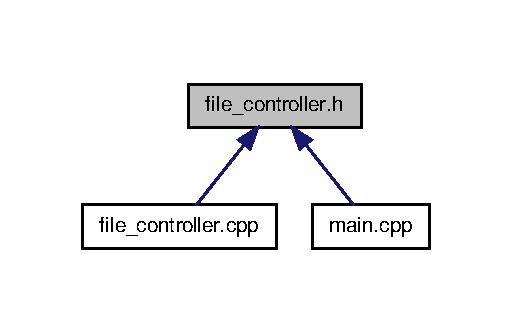
\includegraphics[width=273pt]{file__controller_8h__dep__incl}
\end{center}
\end{figure}
\subsection*{Functions}
\begin{DoxyCompactItemize}
\item 
void \hyperlink{file__controller_8h_aff23a80c6148171c9745ed0c31704e83}{write\-\_\-to\-\_\-file} (string filename, string text, bool secure=true)
\item 
void \hyperlink{file__controller_8h_a90ee1f4929750a48a0e201f8923a2449}{write\-\_\-to\-\_\-file} (string text)
\item 
bool \hyperlink{file__controller_8h_acde73c899ec0618eeb8ae54b0a823f39}{file\-\_\-exists} (const std\-::string \&filename)
\item 
string \hyperlink{file__controller_8h_a5b269a712c2a290dd75694ab5ed3cb18}{read\-\_\-secure\-\_\-filename} ()
\item 
void \hyperlink{file__controller_8h_a8dace9e9ce4bc664cfa4862a21a70c25}{show\-\_\-file} (string filename)
\end{DoxyCompactItemize}


\subsection{Function Documentation}
\hypertarget{file__controller_8h_acde73c899ec0618eeb8ae54b0a823f39}{\index{file\-\_\-controller.\-h@{file\-\_\-controller.\-h}!file\-\_\-exists@{file\-\_\-exists}}
\index{file\-\_\-exists@{file\-\_\-exists}!file_controller.h@{file\-\_\-controller.\-h}}
\subsubsection[{file\-\_\-exists}]{\setlength{\rightskip}{0pt plus 5cm}bool file\-\_\-exists (
\begin{DoxyParamCaption}
\item[{const std\-::string \&}]{filename}
\end{DoxyParamCaption}
)}}\label{file__controller_8h_acde73c899ec0618eeb8ae54b0a823f39}
Checks if a file already exists by its name.


\begin{DoxyParams}{Parameters}
{\em filename} & Filename to check for existence.\\
\hline
\end{DoxyParams}
\begin{DoxyReturn}{Returns}
true when the file exists. false when the file don't exists. 
\end{DoxyReturn}
\hypertarget{file__controller_8h_a5b269a712c2a290dd75694ab5ed3cb18}{\index{file\-\_\-controller.\-h@{file\-\_\-controller.\-h}!read\-\_\-secure\-\_\-filename@{read\-\_\-secure\-\_\-filename}}
\index{read\-\_\-secure\-\_\-filename@{read\-\_\-secure\-\_\-filename}!file_controller.h@{file\-\_\-controller.\-h}}
\subsubsection[{read\-\_\-secure\-\_\-filename}]{\setlength{\rightskip}{0pt plus 5cm}string read\-\_\-secure\-\_\-filename (
\begin{DoxyParamCaption}
{}
\end{DoxyParamCaption}
)}}\label{file__controller_8h_a5b269a712c2a290dd75694ab5ed3cb18}
Promts the user to enter a filename. The filename gets checked for existance. When there is already an existing file for the enterd filename, the user gets promted to override or reenter e new name.

\begin{DoxyReturn}{Returns}
a filename of a new file or of an existing file which can be overwritten. 
\end{DoxyReturn}


Here is the call graph for this function\-:\nopagebreak
\begin{figure}[H]
\begin{center}
\leavevmode
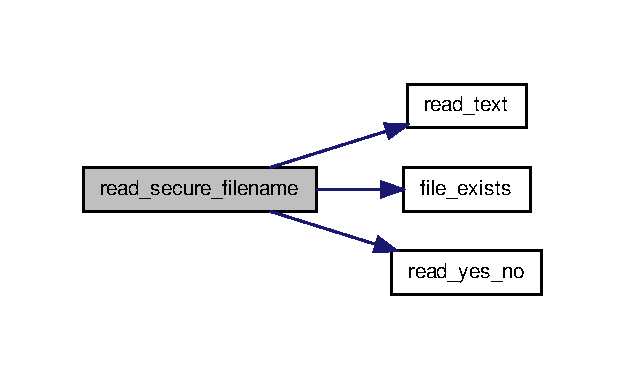
\includegraphics[width=300pt]{file__controller_8h_a5b269a712c2a290dd75694ab5ed3cb18_cgraph}
\end{center}
\end{figure}


\hypertarget{file__controller_8h_a8dace9e9ce4bc664cfa4862a21a70c25}{\index{file\-\_\-controller.\-h@{file\-\_\-controller.\-h}!show\-\_\-file@{show\-\_\-file}}
\index{show\-\_\-file@{show\-\_\-file}!file_controller.h@{file\-\_\-controller.\-h}}
\subsubsection[{show\-\_\-file}]{\setlength{\rightskip}{0pt plus 5cm}void show\-\_\-file (
\begin{DoxyParamCaption}
\item[{string}]{filename}
\end{DoxyParamCaption}
)}}\label{file__controller_8h_a8dace9e9ce4bc664cfa4862a21a70c25}
Reads a file according a given filename and prints the content to the console.


\begin{DoxyParams}{Parameters}
{\em filename} & Name of the file to print to the console. \\
\hline
\end{DoxyParams}
\hypertarget{file__controller_8h_aff23a80c6148171c9745ed0c31704e83}{\index{file\-\_\-controller.\-h@{file\-\_\-controller.\-h}!write\-\_\-to\-\_\-file@{write\-\_\-to\-\_\-file}}
\index{write\-\_\-to\-\_\-file@{write\-\_\-to\-\_\-file}!file_controller.h@{file\-\_\-controller.\-h}}
\subsubsection[{write\-\_\-to\-\_\-file}]{\setlength{\rightskip}{0pt plus 5cm}void write\-\_\-to\-\_\-file (
\begin{DoxyParamCaption}
\item[{string}]{filename, }
\item[{string}]{text, }
\item[{bool}]{secure}
\end{DoxyParamCaption}
)}}\label{file__controller_8h_aff23a80c6148171c9745ed0c31704e83}
Writes given text into a file with the given filename.


\begin{DoxyParams}{Parameters}
{\em filename} & Name of the file to wirte. \\
\hline
{\em text} & Text to write into the file. \\
\hline
\end{DoxyParams}


Here is the call graph for this function\-:\nopagebreak
\begin{figure}[H]
\begin{center}
\leavevmode
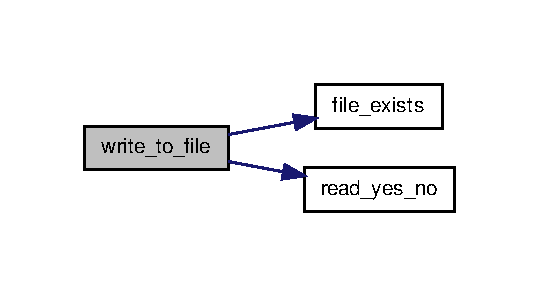
\includegraphics[width=350pt]{file__controller_8h_aff23a80c6148171c9745ed0c31704e83_cgraph}
\end{center}
\end{figure}


\hypertarget{file__controller_8h_a90ee1f4929750a48a0e201f8923a2449}{\index{file\-\_\-controller.\-h@{file\-\_\-controller.\-h}!write\-\_\-to\-\_\-file@{write\-\_\-to\-\_\-file}}
\index{write\-\_\-to\-\_\-file@{write\-\_\-to\-\_\-file}!file_controller.h@{file\-\_\-controller.\-h}}
\subsubsection[{write\-\_\-to\-\_\-file}]{\setlength{\rightskip}{0pt plus 5cm}void write\-\_\-to\-\_\-file (
\begin{DoxyParamCaption}
\item[{string}]{text}
\end{DoxyParamCaption}
)}}\label{file__controller_8h_a90ee1f4929750a48a0e201f8923a2449}
Writes a given text into a file. The name of the file has to be entered by the user. When the file already exists. The user gets prompted to overwrite or entering a new name.


\begin{DoxyParams}{Parameters}
{\em text} & Text to write into the file. \\
\hline
\end{DoxyParams}


Here is the call graph for this function\-:\nopagebreak
\begin{figure}[H]
\begin{center}
\leavevmode
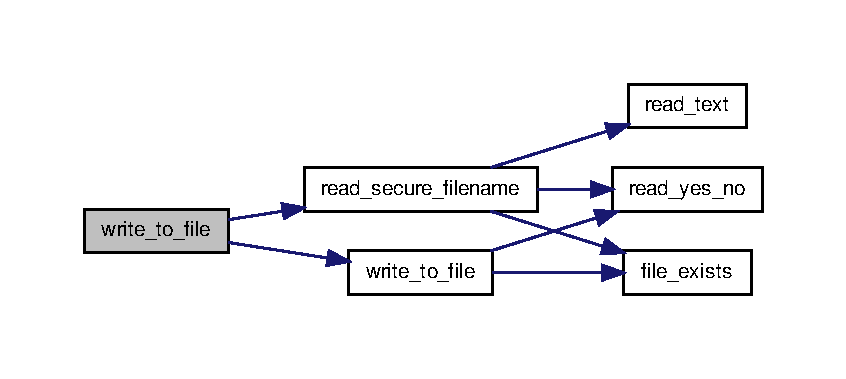
\includegraphics[width=350pt]{file__controller_8h_a90ee1f4929750a48a0e201f8923a2449_cgraph}
\end{center}
\end{figure}



\hypertarget{magic__square_8cpp}{\section{magic\-\_\-square.\-cpp File Reference}
\label{magic__square_8cpp}\index{magic\-\_\-square.\-cpp@{magic\-\_\-square.\-cpp}}
}
{\ttfamily \#include \char`\"{}magic\-\_\-square.\-h\char`\"{}}\\*
{\ttfamily \#include $<$string$>$}\\*
{\ttfamily \#include $<$iostream$>$}\\*
{\ttfamily \#include $<$sstream$>$}\\*
{\ttfamily \#include $<$iomanip$>$}\\*
{\ttfamily \#include $<$stdexcept$>$}\\*
Include dependency graph for magic\-\_\-square.\-cpp\-:\nopagebreak
\begin{figure}[H]
\begin{center}
\leavevmode
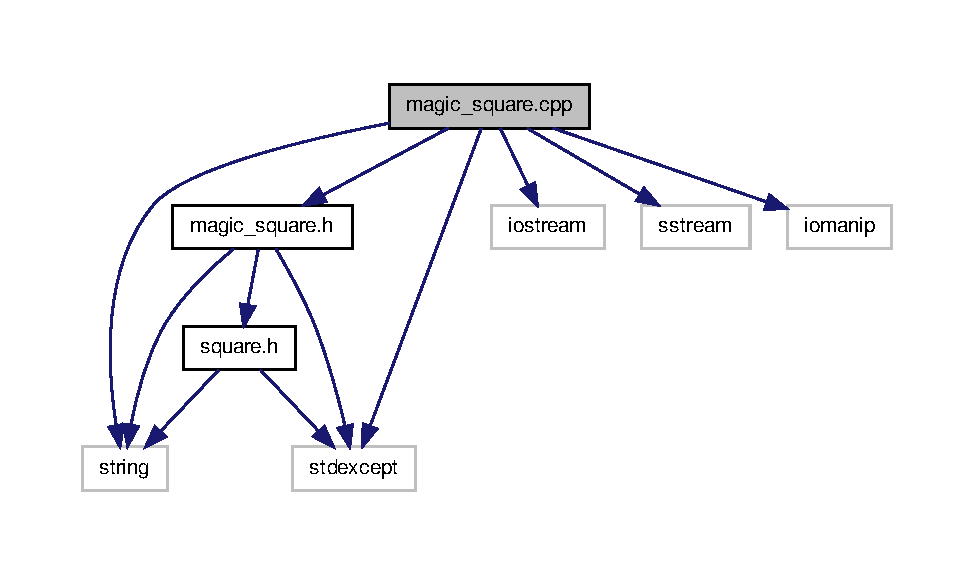
\includegraphics[width=350pt]{magic__square_8cpp__incl}
\end{center}
\end{figure}

\hypertarget{magic__square_8h}{\section{magic\-\_\-square.\-h File Reference}
\label{magic__square_8h}\index{magic\-\_\-square.\-h@{magic\-\_\-square.\-h}}
}
{\ttfamily \#include $<$string$>$}\\*
{\ttfamily \#include $<$stdexcept$>$}\\*
{\ttfamily \#include \char`\"{}square.\-h\char`\"{}}\\*
Include dependency graph for magic\-\_\-square.\-h\-:\nopagebreak
\begin{figure}[H]
\begin{center}
\leavevmode
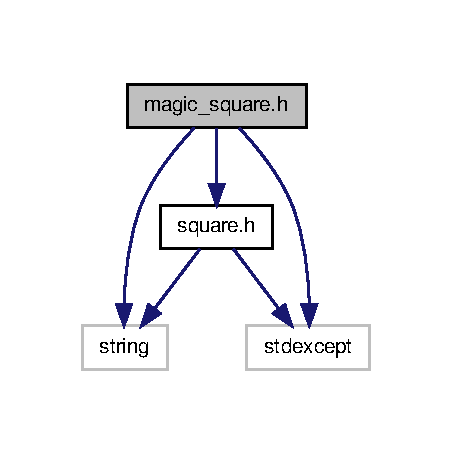
\includegraphics[width=217pt]{magic__square_8h__incl}
\end{center}
\end{figure}
This graph shows which files directly or indirectly include this file\-:\nopagebreak
\begin{figure}[H]
\begin{center}
\leavevmode
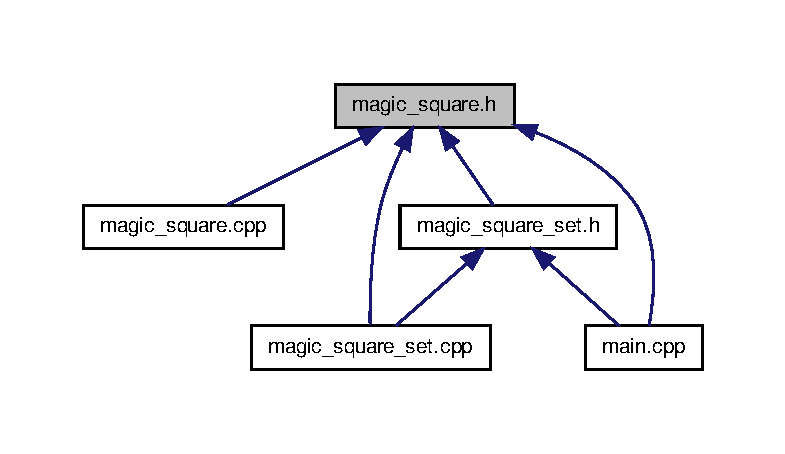
\includegraphics[width=350pt]{magic__square_8h__dep__incl}
\end{center}
\end{figure}
\subsection*{Classes}
\begin{DoxyCompactItemize}
\item 
class \hyperlink{classMagicSquare}{Magic\-Square}
\end{DoxyCompactItemize}

\hypertarget{magic__square__set_8cpp}{\section{magic\-\_\-square\-\_\-set.\-cpp File Reference}
\label{magic__square__set_8cpp}\index{magic\-\_\-square\-\_\-set.\-cpp@{magic\-\_\-square\-\_\-set.\-cpp}}
}
{\ttfamily \#include \char`\"{}magic\-\_\-square\-\_\-set.\-h\char`\"{}}\\*
{\ttfamily \#include \char`\"{}magic\-\_\-square.\-h\char`\"{}}\\*
{\ttfamily \#include $<$iostream$>$}\\*
{\ttfamily \#include $<$sstream$>$}\\*
{\ttfamily \#include $<$iomanip$>$}\\*
{\ttfamily \#include $<$vector$>$}\\*
Include dependency graph for magic\-\_\-square\-\_\-set.\-cpp\-:\nopagebreak
\begin{figure}[H]
\begin{center}
\leavevmode
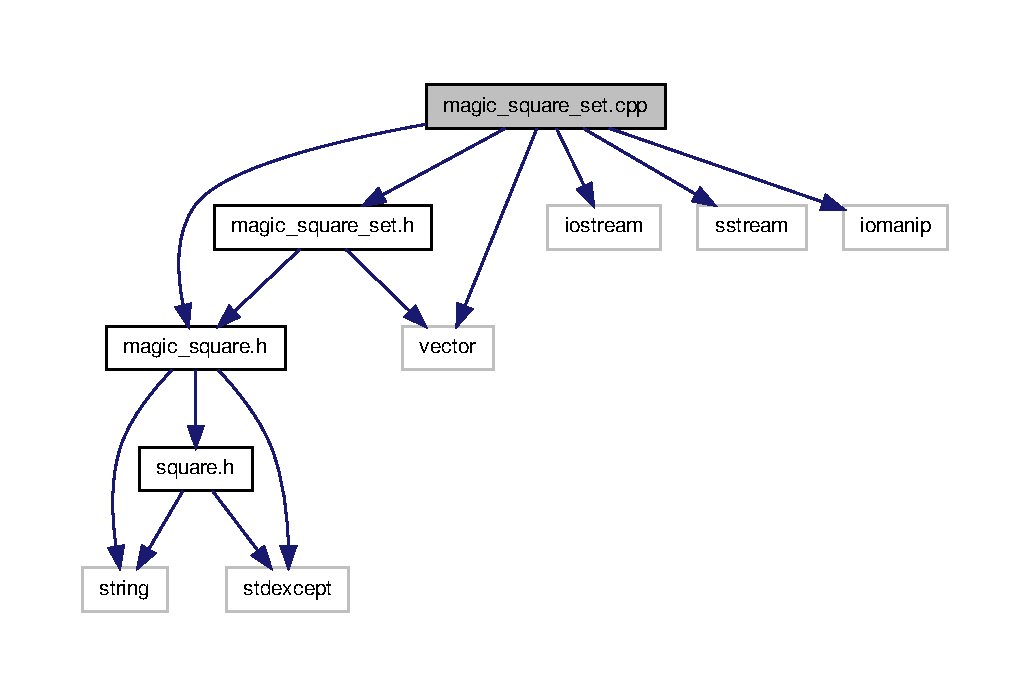
\includegraphics[width=350pt]{magic__square__set_8cpp__incl}
\end{center}
\end{figure}

\hypertarget{magic__square__set_8h}{\section{magic\-\_\-square\-\_\-set.\-h File Reference}
\label{magic__square__set_8h}\index{magic\-\_\-square\-\_\-set.\-h@{magic\-\_\-square\-\_\-set.\-h}}
}
{\ttfamily \#include \char`\"{}magic\-\_\-square.\-h\char`\"{}}\\*
{\ttfamily \#include $<$vector$>$}\\*
Include dependency graph for magic\-\_\-square\-\_\-set.\-h\-:\nopagebreak
\begin{figure}[H]
\begin{center}
\leavevmode
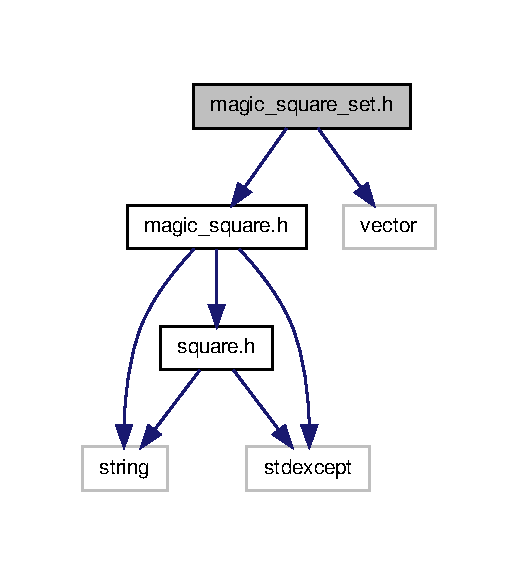
\includegraphics[width=249pt]{magic__square__set_8h__incl}
\end{center}
\end{figure}
This graph shows which files directly or indirectly include this file\-:\nopagebreak
\begin{figure}[H]
\begin{center}
\leavevmode
\includegraphics[width=268pt]{magic__square__set_8h__dep__incl}
\end{center}
\end{figure}
\subsection*{Classes}
\begin{DoxyCompactItemize}
\item 
class \hyperlink{classMagicSquareSet}{Magic\-Square\-Set}
\end{DoxyCompactItemize}

\hypertarget{main_8cpp}{\section{main.\-cpp File Reference}
\label{main_8cpp}\index{main.\-cpp@{main.\-cpp}}
}
{\ttfamily \#include $<$iostream$>$}\\*
{\ttfamily \#include $<$iomanip$>$}\\*
{\ttfamily \#include $<$string$>$}\\*
{\ttfamily \#include \char`\"{}maumau.\-h\char`\"{}}\\*
Include dependency graph for main.\-cpp\-:\nopagebreak
\begin{figure}[H]
\begin{center}
\leavevmode
\includegraphics[width=350pt]{main_8cpp__incl}
\end{center}
\end{figure}
\subsection*{Functions}
\begin{DoxyCompactItemize}
\item 
void \hyperlink{main_8cpp_ad45e149aada26b44cb0274a5eb865edb}{print\-\_\-manual} ()
\item 
int \hyperlink{main_8cpp_a0ddf1224851353fc92bfbff6f499fa97}{main} (int argc, char $\ast$argv\mbox{[}$\,$\mbox{]})
\end{DoxyCompactItemize}


\subsection{Function Documentation}
\hypertarget{main_8cpp_a0ddf1224851353fc92bfbff6f499fa97}{\index{main.\-cpp@{main.\-cpp}!main@{main}}
\index{main@{main}!main.cpp@{main.\-cpp}}
\subsubsection[{main}]{\setlength{\rightskip}{0pt plus 5cm}int main (
\begin{DoxyParamCaption}
\item[{int}]{argc, }
\item[{char $\ast$}]{argv\mbox{[}$\,$\mbox{]}}
\end{DoxyParamCaption}
)}}\label{main_8cpp_a0ddf1224851353fc92bfbff6f499fa97}
Entrypoint to the program \char`\"{}\-Maumau\char`\"{}. Checks the arguments given by the user and starts a new game for four players. When the option -\/a is set the game gets completely simulated. When the option -\/m is set the User will play the \hyperlink{classPlayer}{Player} 1. If the program gets started with invalid parameters, there is a manual shown. 

Here is the call graph for this function\-:\nopagebreak
\begin{figure}[H]
\begin{center}
\leavevmode
\includegraphics[width=350pt]{main_8cpp_a0ddf1224851353fc92bfbff6f499fa97_cgraph}
\end{center}
\end{figure}


\hypertarget{main_8cpp_ad45e149aada26b44cb0274a5eb865edb}{\index{main.\-cpp@{main.\-cpp}!print\-\_\-manual@{print\-\_\-manual}}
\index{print\-\_\-manual@{print\-\_\-manual}!main.cpp@{main.\-cpp}}
\subsubsection[{print\-\_\-manual}]{\setlength{\rightskip}{0pt plus 5cm}void print\-\_\-manual (
\begin{DoxyParamCaption}
{}
\end{DoxyParamCaption}
)}}\label{main_8cpp_ad45e149aada26b44cb0274a5eb865edb}

\hypertarget{square_8cpp}{\section{square.\-cpp File Reference}
\label{square_8cpp}\index{square.\-cpp@{square.\-cpp}}
}
{\ttfamily \#include \char`\"{}square.\-h\char`\"{}}\\*
{\ttfamily \#include $<$string$>$}\\*
{\ttfamily \#include $<$sstream$>$}\\*
{\ttfamily \#include $<$cstdlib$>$}\\*
Include dependency graph for square.\-cpp\-:\nopagebreak
\begin{figure}[H]
\begin{center}
\leavevmode
\includegraphics[width=314pt]{square_8cpp__incl}
\end{center}
\end{figure}

\hypertarget{square_8h}{\section{square.\-h File Reference}
\label{square_8h}\index{square.\-h@{square.\-h}}
}
{\ttfamily \#include $<$string$>$}\\*
{\ttfamily \#include $<$stdexcept$>$}\\*
Include dependency graph for square.\-h\-:\nopagebreak
\begin{figure}[H]
\begin{center}
\leavevmode
\includegraphics[width=196pt]{square_8h__incl}
\end{center}
\end{figure}
This graph shows which files directly or indirectly include this file\-:\nopagebreak
\begin{figure}[H]
\begin{center}
\leavevmode
\includegraphics[width=350pt]{square_8h__dep__incl}
\end{center}
\end{figure}
\subsection*{Classes}
\begin{DoxyCompactItemize}
\item 
class \hyperlink{classSquare}{Square}
\end{DoxyCompactItemize}

\addcontentsline{toc}{part}{Index}
\printindex
\end{document}
